\documentclass[11pt]{article}
\usepackage[margin = 1in]{geometry}
\usepackage{amsmath}
\usepackage{amssymb}
\usepackage{amsthm}
\usepackage{graphicx}
\usepackage{enumitem}
\usepackage{url}
\usepackage[parfill]{parskip}
\usepackage{listings}
\newcommand{\skipline}{\vspace{\baselineskip}}
\newcommand{\spacer}{\noalign{\medskip}}
\newenvironment{problem}[1]{\textbf{Problem #1:}}{\newpage}
\usepackage{caption}
\usepackage{subcaption}
\usepackage[utf8]{inputenc}
\usepackage{xcolor}
\definecolor{codegreen}{rgb}{0,0.6,0}
\definecolor{codegray}{rgb}{0.5,0.5,0.5}
\definecolor{codepurple}{rgb}{0.58,0,0.82}
\definecolor{backcolour}{rgb}{0.95,0.95,0.92}
\lstdefinestyle{mystyle}{
	backgroundcolor=\color{backcolour},   
	commentstyle=\color{codegreen},
	keywordstyle=\color{magenta},
	numberstyle=\tiny\color{codegray},
	stringstyle=\color{codepurple},
	basicstyle=\ttfamily\footnotesize,
	breakatwhitespace=false,         
	breaklines=true,                 
	captionpos=b,                    
	keepspaces=true,                 
	numbers=left,                    
	numbersep=5pt,                  
	showspaces=false,                
	showstringspaces=false,
	showtabs=false,                  
	tabsize=2
}
\lstset{style=mystyle}
% Options for packages loaded elsewhere
\PassOptionsToPackage{unicode}{hyperref}
\PassOptionsToPackage{hyphens}{url}
%
\usepackage{lmodern}
\usepackage{amssymb,amsmath}
\usepackage{ifxetex,ifluatex}
\ifnum 0\ifxetex 1\fi\ifluatex 1\fi=0 % if pdftex
\usepackage[T1]{fontenc}
\usepackage[utf8]{inputenc}
\usepackage{textcomp} % provide euro and other symbols
\else % if luatex or xetex
\usepackage{unicode-math}
\defaultfontfeatures{Scale=MatchLowercase}
\defaultfontfeatures[\rmfamily]{Ligatures=TeX,Scale=1}
\fi
% Use upquote if available, for straight quotes in verbatim environments
\IfFileExists{upquote.sty}{\usepackage{upquote}}{}
\IfFileExists{microtype.sty}{% use microtype if available
	\usepackage[]{microtype}
	\UseMicrotypeSet[protrusion]{basicmath} % disable protrusion for tt fonts
}{}
\makeatletter
\@ifundefined{KOMAClassName}{% if non-KOMA class
	\IfFileExists{parskip.sty}{%
		\usepackage{parskip}
	}{% else
		\setlength{\parindent}{0pt}
		\setlength{\parskip}{6pt plus 2pt minus 1pt}}
}{% if KOMA class
	\KOMAoptions{parskip=half}}
\makeatother
\usepackage{xcolor}
\IfFileExists{xurl.sty}{\usepackage{xurl}}{} % add URL line breaks if available
\IfFileExists{bookmark.sty}{\usepackage{bookmark}}{\usepackage{hyperref}}
\hypersetup{
	hidelinks,
	pdfcreator={LaTeX via pandoc}}
\urlstyle{same} % disable monospaced font for URLs
\usepackage[margin=1in]{geometry}
\usepackage{color}
\usepackage{fancyvrb}
\newcommand{\VerbBar}{|}
\newcommand{\VERB}{\Verb[commandchars=\\\{\}]}
\DefineVerbatimEnvironment{Highlighting}{Verbatim}{commandchars=\\\{\}}
% Add ',fontsize=\small' for more characters per line
\usepackage{framed}
\definecolor{shadecolor}{RGB}{248,248,248}
\newenvironment{Shaded}{\begin{snugshade}}{\end{snugshade}}
\newcommand{\AlertTok}[1]{\textcolor[rgb]{0.94,0.16,0.16}{#1}}
\newcommand{\AnnotationTok}[1]{\textcolor[rgb]{0.56,0.35,0.01}{\textbf{\textit{#1}}}}
\newcommand{\AttributeTok}[1]{\textcolor[rgb]{0.77,0.63,0.00}{#1}}
\newcommand{\BaseNTok}[1]{\textcolor[rgb]{0.00,0.00,0.81}{#1}}
\newcommand{\BuiltInTok}[1]{#1}
\newcommand{\CharTok}[1]{\textcolor[rgb]{0.31,0.60,0.02}{#1}}
\newcommand{\CommentTok}[1]{\textcolor[rgb]{0.56,0.35,0.01}{\textit{#1}}}
\newcommand{\CommentVarTok}[1]{\textcolor[rgb]{0.56,0.35,0.01}{\textbf{\textit{#1}}}}
\newcommand{\ConstantTok}[1]{\textcolor[rgb]{0.00,0.00,0.00}{#1}}
\newcommand{\ControlFlowTok}[1]{\textcolor[rgb]{0.13,0.29,0.53}{\textbf{#1}}}
\newcommand{\DataTypeTok}[1]{\textcolor[rgb]{0.13,0.29,0.53}{#1}}
\newcommand{\DecValTok}[1]{\textcolor[rgb]{0.00,0.00,0.81}{#1}}
\newcommand{\DocumentationTok}[1]{\textcolor[rgb]{0.56,0.35,0.01}{\textbf{\textit{#1}}}}
\newcommand{\ErrorTok}[1]{\textcolor[rgb]{0.64,0.00,0.00}{\textbf{#1}}}
\newcommand{\ExtensionTok}[1]{#1}
\newcommand{\FloatTok}[1]{\textcolor[rgb]{0.00,0.00,0.81}{#1}}
\newcommand{\FunctionTok}[1]{\textcolor[rgb]{0.00,0.00,0.00}{#1}}
\newcommand{\ImportTok}[1]{#1}
\newcommand{\InformationTok}[1]{\textcolor[rgb]{0.56,0.35,0.01}{\textbf{\textit{#1}}}}
\newcommand{\KeywordTok}[1]{\textcolor[rgb]{0.13,0.29,0.53}{\textbf{#1}}}
\newcommand{\NormalTok}[1]{#1}
\newcommand{\OperatorTok}[1]{\textcolor[rgb]{0.81,0.36,0.00}{\textbf{#1}}}
\newcommand{\OtherTok}[1]{\textcolor[rgb]{0.56,0.35,0.01}{#1}}
\newcommand{\PreprocessorTok}[1]{\textcolor[rgb]{0.56,0.35,0.01}{\textit{#1}}}
\newcommand{\RegionMarkerTok}[1]{#1}
\newcommand{\SpecialCharTok}[1]{\textcolor[rgb]{0.00,0.00,0.00}{#1}}
\newcommand{\SpecialStringTok}[1]{\textcolor[rgb]{0.31,0.60,0.02}{#1}}
\newcommand{\StringTok}[1]{\textcolor[rgb]{0.31,0.60,0.02}{#1}}
\newcommand{\VariableTok}[1]{\textcolor[rgb]{0.00,0.00,0.00}{#1}}
\newcommand{\VerbatimStringTok}[1]{\textcolor[rgb]{0.31,0.60,0.02}{#1}}
\newcommand{\WarningTok}[1]{\textcolor[rgb]{0.56,0.35,0.01}{\textbf{\textit{#1}}}}
\usepackage{graphicx,grffile}
\makeatletter
\def\maxwidth{\ifdim\Gin@nat@width>\linewidth\linewidth\else\Gin@nat@width\fi}
\def\maxheight{\ifdim\Gin@nat@height>\textheight\textheight\else\Gin@nat@height\fi}
\makeatother
% Scale images if necessary, so that they will not overflow the page
% margins by default, and it is still possible to overwrite the defaults
% using explicit options in \includegraphics[width, height, ...]{}
\setkeys{Gin}{width=\maxwidth,height=\maxheight,keepaspectratio}
% Set default figure placement to htbp
\makeatletter
\def\fps@figure{htbp}
\makeatother
\setlength{\emergencystretch}{3em} % prevent overfull lines
\providecommand{\tightlist}{%
	\setlength{\itemsep}{0pt}\setlength{\parskip}{0pt}}
\setcounter{secnumdepth}{-\maxdimen} % remove section numbering


\begin{document}
	
	\begin{center}
		\textbf{Homework 3} \\
		\textbf{Intro Math Modeling} \\
		\textbf{Math 336} \\
		\textbf{Stephen Giang RedID: 823184070} \\
		\skipline \skipline
	\end{center}

	\begin{problem}{1-2 Exercise (5.8)}
		Make an SVD space-time data decomposition for the $5^\circ \times 5^\circ$
		latitude-longitude gridded annual (July-June) mean sea surface temperature field anomalies from 1951-2000 over
		the tropical Pacific: ($20^\circ S -20^\circ N, 160^\circ E -100^\circ W$). The dataset is posted on the course
		blackboard. 
		\begin{enumerate}[label = (\alph*)]
			\item Perform the SVD analysis for the data. Print out the first 10 eigenvalues.
			\\ \\
			Notice the first 10 eigenvalues can be found by $\lambda_i = \frac{d_i^2}{t}$
			\begin{figure}[h!]
				\centering
				\begin{tabular}{|c|c|c|c|c|}
					\hline
					27.7879120 & 4.3773517 & 2.5610076 & 0.9341387 & 0.6615021 \\
					0.4678065 & 0.3243314 & 0.2490007 & 0.1680932 & 0.1443271 \\
					\hline
				\end{tabular}
			\end{figure}
			
\begin{Shaded}
\begin{Highlighting}[]
\CommentTok{# Problem 1-2}

\KeywordTok{setwd}\NormalTok{(}\StringTok{'C:/Users/Stephen Giang/Documents/Math336Files/data'}\NormalTok{)}
\NormalTok{readData =}\StringTok{ }\KeywordTok{read.csv}\NormalTok{(}\StringTok{'NOAAGlobalT.csv'}\NormalTok{)}

\NormalTok{pacific1 =}\StringTok{ }\KeywordTok{subset}\NormalTok{(readData, LAT }\OperatorTok{>=}\StringTok{ }\DecValTok{-20} \OperatorTok{&}\StringTok{ }\NormalTok{LAT }\OperatorTok{<=}\StringTok{ }\DecValTok{20}\NormalTok{)   }\CommentTok{#20S  - 20N}
\NormalTok{pacific1 =}\StringTok{ }\KeywordTok{subset}\NormalTok{(pacific1, LON }\OperatorTok{>=}\StringTok{ }\DecValTok{160} \OperatorTok{&}\StringTok{ }\NormalTok{LON }\OperatorTok{<=}\StringTok{ }\DecValTok{260}\NormalTok{)  }\CommentTok{#160E - 100W}
\NormalTok{pacific1 =}\StringTok{ }\NormalTok{pacific1[, }\DecValTok{856}\OperatorTok{:}\DecValTok{1455}\NormalTok{]   }\CommentTok{# 01/1951 - 12/2000}

\CommentTok{# -999.9 means missing data so set to 0}
\ControlFlowTok{for}\NormalTok{ ( i }\ControlFlowTok{in} \DecValTok{1}\OperatorTok{:}\KeywordTok{dim}\NormalTok{(pacific1)[}\DecValTok{1}\NormalTok{] ) \{}
  \ControlFlowTok{for}\NormalTok{ ( j }\ControlFlowTok{in} \DecValTok{1}\OperatorTok{:}\KeywordTok{dim}\NormalTok{(pacific1)[}\DecValTok{2}\NormalTok{] ) \{}
    \ControlFlowTok{if}\NormalTok{ (pacific1[i,j] }\OperatorTok{<}\StringTok{ }\DecValTok{-800}\NormalTok{) \{}
\NormalTok{      pacific1[i,j] =}\StringTok{ }\DecValTok{0}
\NormalTok{    \}}
\NormalTok{  \}}
\NormalTok{\}}

\NormalTok{yearDiff =}\StringTok{ }\DecValTok{1999} \OperatorTok{-}\StringTok{ }\DecValTok{1951}\OperatorTok{+}\StringTok{ }\DecValTok{1} 
\NormalTok{pacific =}\StringTok{ }\KeywordTok{matrix}\NormalTok{(}\DecValTok{0}\NormalTok{,}\DataTypeTok{nrow =} \KeywordTok{dim}\NormalTok{(pacific1)[}\DecValTok{1}\NormalTok{], }\DataTypeTok{ncol =}\NormalTok{ yearDiff)}
\CommentTok{# Annual (July - June) Mean Sea Temp}
\ControlFlowTok{for}\NormalTok{ (k }\ControlFlowTok{in} \DecValTok{1}\OperatorTok{:}\NormalTok{yearDiff) \{}
\NormalTok{  pacific[, k] =}\StringTok{ }\KeywordTok{rowMeans}\NormalTok{(pacific1[, (}\DecValTok{12}\OperatorTok{*}\NormalTok{k }\OperatorTok{-}\StringTok{ }\DecValTok{5}\NormalTok{) }\OperatorTok{:}\StringTok{ }\NormalTok{(}\DecValTok{12}\OperatorTok{*}\NormalTok{k }\OperatorTok{+}\StringTok{ }\DecValTok{6}\NormalTok{) ])}
\NormalTok{\}}
\end{Highlighting}
\end{Shaded}
\newpage
\begin{Shaded}
\begin{Highlighting}[]
\NormalTok{svdPacific =}\StringTok{ }\KeywordTok{svd}\NormalTok{(pacific)}
\NormalTok{D =}\StringTok{ }\KeywordTok{diag}\NormalTok{(svdPacific}\OperatorTok{$}\NormalTok{d)}
\NormalTok{U =}\StringTok{ }\NormalTok{svdPacific}\OperatorTok{$}\NormalTok{u}
\NormalTok{V =}\StringTok{ }\NormalTok{svdPacific}\OperatorTok{$}\NormalTok{v}

\NormalTok{eigVals =}\StringTok{ }\NormalTok{(svdPacific}\OperatorTok{$}\NormalTok{d[}\DecValTok{1}\OperatorTok{:}\DecValTok{10}\NormalTok{])}\OperatorTok{^}\DecValTok{2} \OperatorTok{/}\StringTok{ }\NormalTok{yearDiff}
\NormalTok{eigVals}
\end{Highlighting}
\end{Shaded}
			
\begin{verbatim}
##  [1] 27.7879120  4.3773517  2.5610076  0.9341387  0.6615021  
##  [6]  0.4678065  0.3243314  0.2490007  0.1680932  0.1443271
\end{verbatim}

\newpage
\item Plot the map of the first three U column vectors, which are the spatial patterns of the
data field, and are also known as Empirical Orthogonal Functions (EOFs).

\begin{Shaded}
\begin{Highlighting}[]
\NormalTok{x =}\StringTok{ }\KeywordTok{seq}\NormalTok{(}\OperatorTok{-}\FloatTok{17.5}\NormalTok{, }\FloatTok{17.5}\NormalTok{, }\DataTypeTok{by=}\DecValTok{5}\NormalTok{)  }\CommentTok{# lat}
\NormalTok{y =}\StringTok{ }\KeywordTok{seq}\NormalTok{(}\FloatTok{162.5}\NormalTok{, }\FloatTok{257.5}\NormalTok{, }\DataTypeTok{by=}\DecValTok{5}\NormalTok{) }\CommentTok{# lon}
\NormalTok{numLatVals =}\StringTok{ }\KeywordTok{length}\NormalTok{(x)}
\NormalTok{numLonVals =}\StringTok{ }\KeywordTok{length}\NormalTok{(y)}
\NormalTok{time =}\StringTok{ }\DecValTok{1951} \OperatorTok{:}\StringTok{ }\DecValTok{1999}

\NormalTok{int=}\KeywordTok{seq}\NormalTok{(}\OperatorTok{-}\FloatTok{0.2}\NormalTok{,}\FloatTok{0.2}\NormalTok{,}\DataTypeTok{length.out=}\DecValTok{81}\NormalTok{)}
\NormalTok{rgb.palette=}\KeywordTok{colorRampPalette}\NormalTok{(}\KeywordTok{c}\NormalTok{(}\StringTok{'black'}\NormalTok{,}\StringTok{'blue'}\NormalTok{, }\StringTok{'darkgreen'}\NormalTok{,}
                               \StringTok{'green'}\NormalTok{, }\StringTok{'yellow'}\NormalTok{,}\StringTok{'pink'}\NormalTok{,}\StringTok{'red'}\NormalTok{,}\StringTok{'maroon'}\NormalTok{),}
                               \DataTypeTok{interpolate=}\StringTok{'spline'}\NormalTok{)}
\KeywordTok{suppressWarnings}\NormalTok{(}\KeywordTok{library}\NormalTok{(maps))}
\end{Highlighting}
\end{Shaded}
			
\begin{Shaded}
\begin{Highlighting}
\NormalTok{umat =}\StringTok{ }\KeywordTok{matrix}\NormalTok{(U[,}\DecValTok{1}\NormalTok{], }\DataTypeTok{nrow =}\NormalTok{ numLonVals)}
\KeywordTok{filled.contour}\NormalTok{(y, x, umat, }\DataTypeTok{color.palette=}\NormalTok{rgb.palette, }\DataTypeTok{levels=}\NormalTok{int,}
               \DataTypeTok{xlim=}\KeywordTok{c}\NormalTok{(}\DecValTok{120}\NormalTok{,}\DecValTok{300}\NormalTok{),}\DataTypeTok{ylim=}\KeywordTok{c}\NormalTok{(}\OperatorTok{-}\DecValTok{40}\NormalTok{,}\DecValTok{40}\NormalTok{),}
               \DataTypeTok{plot.title=}\KeywordTok{title}\NormalTok{(}\DataTypeTok{main=}\StringTok{"EOF1 of the Tropical Pacific Temp Data"}\NormalTok{,}
                                \DataTypeTok{xlab=}\StringTok{"Latitude"}\NormalTok{,}\DataTypeTok{ylab=}\StringTok{"Longitude"}\NormalTok{),}
               \DataTypeTok{plot.axes=}\NormalTok{\{}\KeywordTok{axis}\NormalTok{(}\DecValTok{1}\NormalTok{); }\KeywordTok{axis}\NormalTok{(}\DecValTok{2}\NormalTok{); }\KeywordTok{map}\NormalTok{(}\StringTok{'world2'}\NormalTok{, }\DataTypeTok{add=}\OtherTok{TRUE}\NormalTok{); }\KeywordTok{grid}\NormalTok{()\},}
               \DataTypeTok{key.title=}\KeywordTok{title}\NormalTok{(}\DataTypeTok{main=}\StringTok{"[oC]"}\NormalTok{))}
\end{Highlighting}
\end{Shaded}

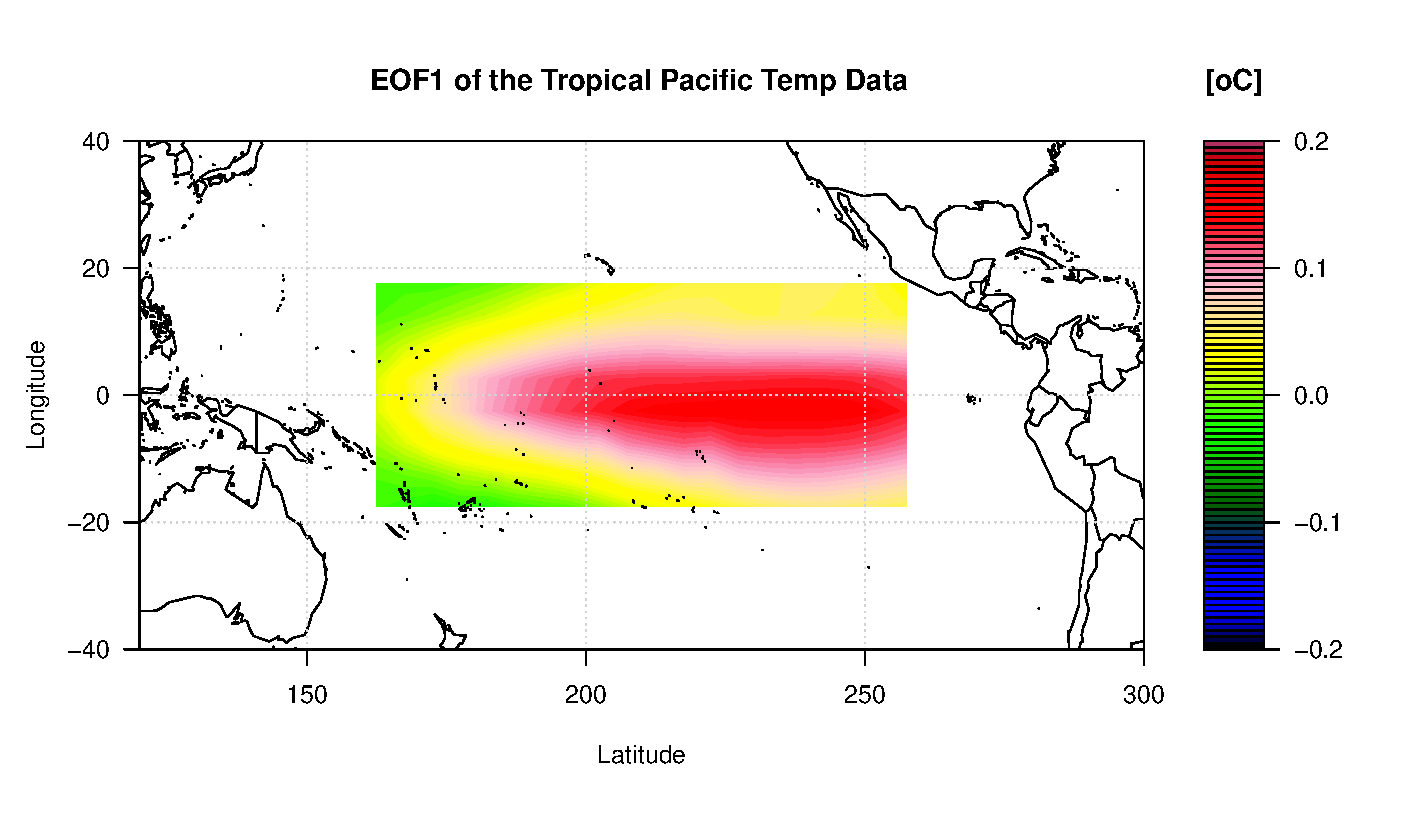
\includegraphics[height = 8cm]{Figures/Prob1/EOF1}

\newpage
\begin{Shaded}
\begin{Highlighting}[]
\NormalTok{umat =}\StringTok{ }\KeywordTok{matrix}\NormalTok{(U[,}\DecValTok{2}\NormalTok{], }\DataTypeTok{nrow =}\NormalTok{ numLonVals)}
\KeywordTok{filled.contour}\NormalTok{(y, x, umat, }\DataTypeTok{color.palette=}\NormalTok{rgb.palette, }\DataTypeTok{levels=}\NormalTok{int,}
               \DataTypeTok{xlim=}\KeywordTok{c}\NormalTok{(}\DecValTok{120}\NormalTok{,}\DecValTok{300}\NormalTok{),}\DataTypeTok{ylim=}\KeywordTok{c}\NormalTok{(}\OperatorTok{-}\DecValTok{40}\NormalTok{,}\DecValTok{40}\NormalTok{),}
               \DataTypeTok{plot.title=}\KeywordTok{title}\NormalTok{(}\DataTypeTok{main=}\StringTok{"EOF2 of the Tropical Pacific Temp Data"}\NormalTok{,}
                                \DataTypeTok{xlab=}\StringTok{"Latitude"}\NormalTok{,}\DataTypeTok{ylab=}\StringTok{"Longitude"}\NormalTok{),}
               \DataTypeTok{plot.axes=}\NormalTok{\{}\KeywordTok{axis}\NormalTok{(}\DecValTok{1}\NormalTok{); }\KeywordTok{axis}\NormalTok{(}\DecValTok{2}\NormalTok{); }\KeywordTok{map}\NormalTok{(}\StringTok{'world2'}\NormalTok{, }\DataTypeTok{add=}\OtherTok{TRUE}\NormalTok{); }\KeywordTok{grid}\NormalTok{()\},}
               \DataTypeTok{key.title=}\KeywordTok{title}\NormalTok{(}\DataTypeTok{main=}\StringTok{"[oC]"}\NormalTok{))}
\end{Highlighting}
\end{Shaded}
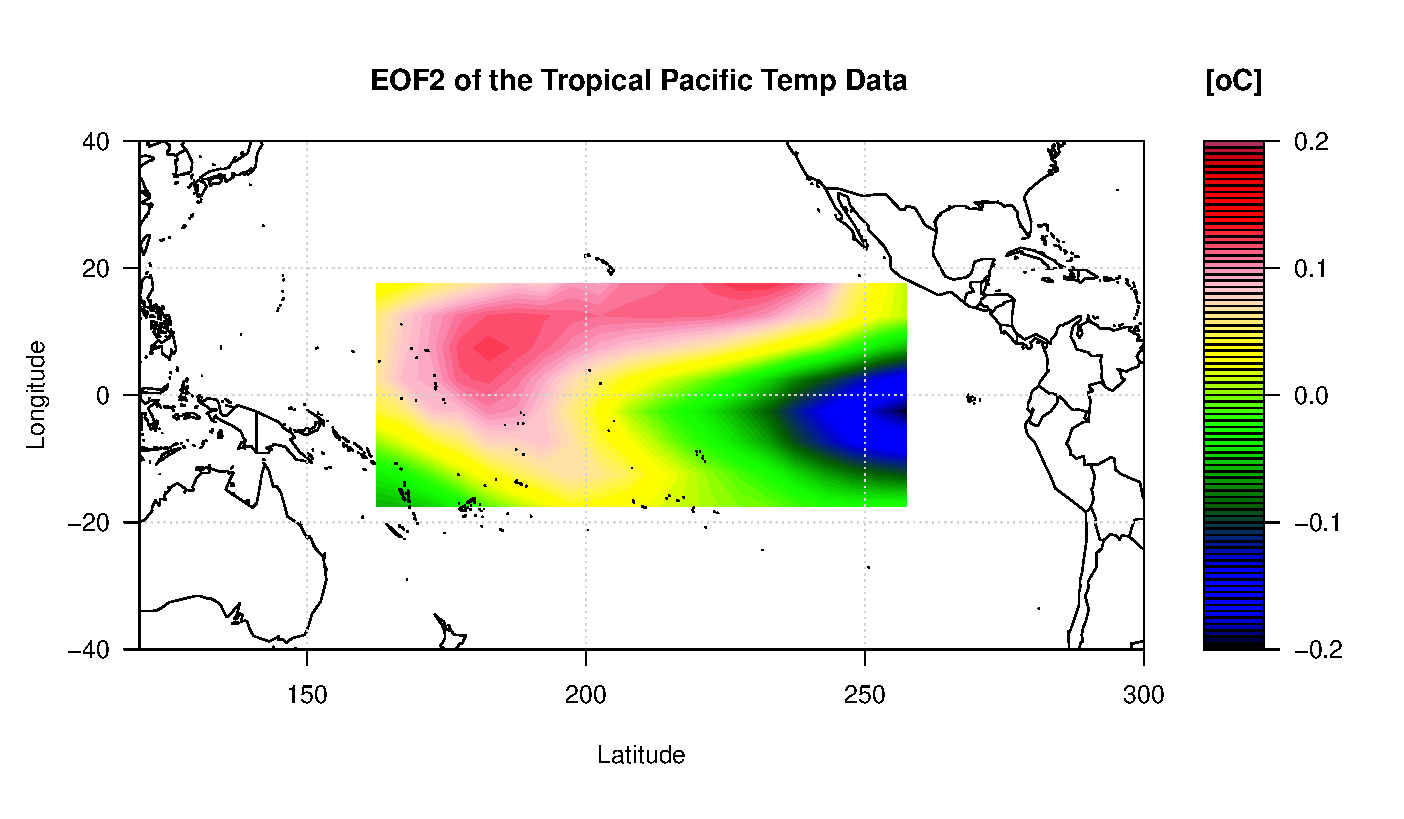
\includegraphics[height = 7.5cm]{Figures/Prob1/EOF2}
\begin{Shaded}
\begin{Highlighting}[]
\NormalTok{umat =}\StringTok{ }\KeywordTok{matrix}\NormalTok{(U[,}\DecValTok{3}\NormalTok{], }\DataTypeTok{nrow =}\NormalTok{ numLonVals)}
\KeywordTok{filled.contour}\NormalTok{(y, x, umat, }\DataTypeTok{color.palette=}\NormalTok{rgb.palette, }\DataTypeTok{levels=}\NormalTok{int,}
               \DataTypeTok{xlim=}\KeywordTok{c}\NormalTok{(}\DecValTok{120}\NormalTok{,}\DecValTok{300}\NormalTok{),}\DataTypeTok{ylim=}\KeywordTok{c}\NormalTok{(}\OperatorTok{-}\DecValTok{40}\NormalTok{,}\DecValTok{40}\NormalTok{),}
               \DataTypeTok{plot.title=}\KeywordTok{title}\NormalTok{(}\DataTypeTok{main=}\StringTok{"EOF3 of the Tropical Pacific Temp Data"}\NormalTok{,}
                                \DataTypeTok{xlab=}\StringTok{"Latitude"}\NormalTok{,}\DataTypeTok{ylab=}\StringTok{"Longitude"}\NormalTok{),}
               \DataTypeTok{plot.axes=}\NormalTok{\{}\KeywordTok{axis}\NormalTok{(}\DecValTok{1}\NormalTok{); }\KeywordTok{axis}\NormalTok{(}\DecValTok{2}\NormalTok{); }\KeywordTok{map}\NormalTok{(}\StringTok{'world2'}\NormalTok{, }\DataTypeTok{add=}\OtherTok{TRUE}\NormalTok{); }\KeywordTok{grid}\NormalTok{()\},}
               \DataTypeTok{key.title=}\KeywordTok{title}\NormalTok{(}\DataTypeTok{main=}\StringTok{"[oC]"}\NormalTok{))}
\end{Highlighting}
\end{Shaded}
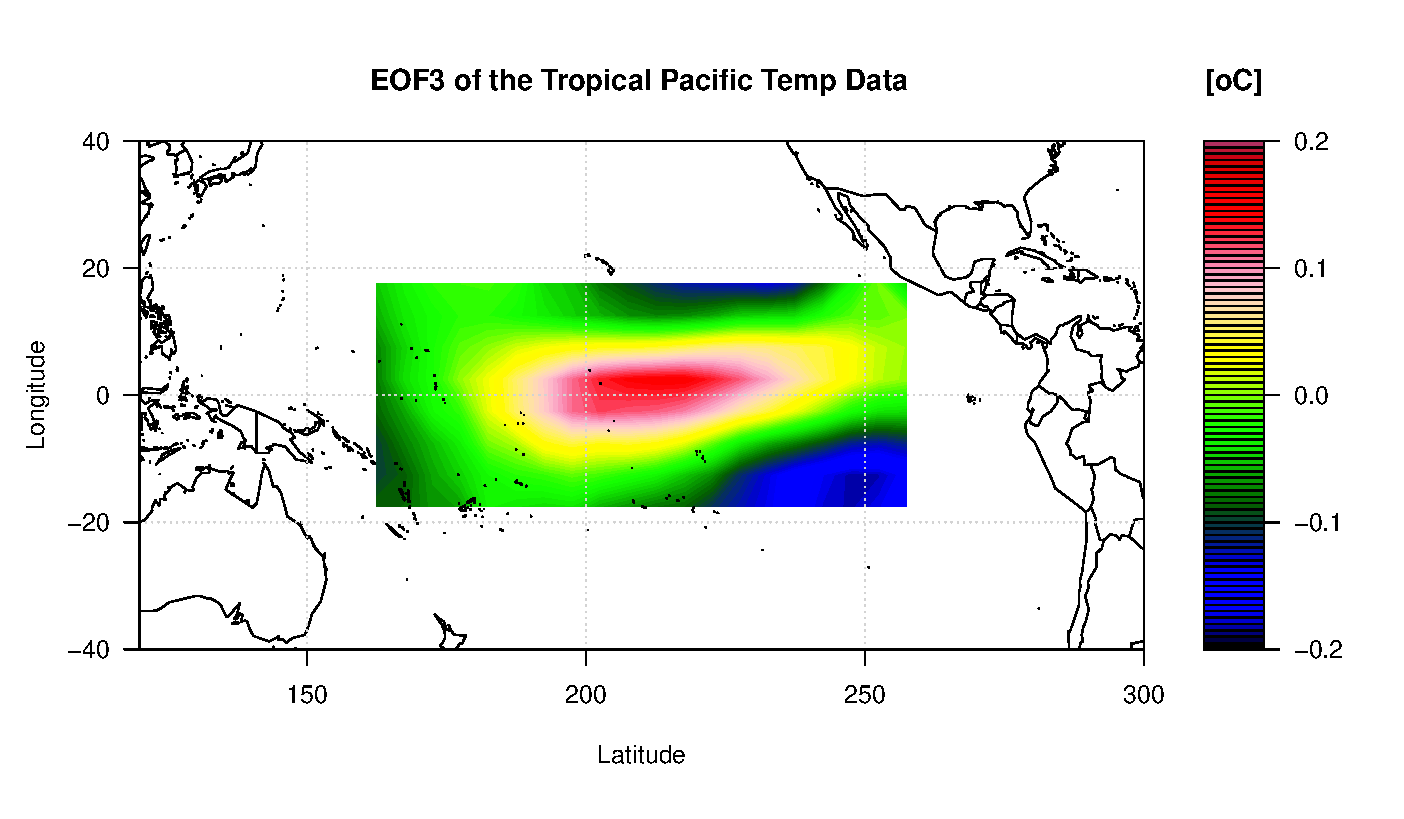
\includegraphics[height = 7.5cm]{Figures/Prob1/EOF3}

\item Plot the time series of the first three V column vectors, which are the temporal patterns
of the data field, and are also known as Principal Components (PCs).

\begin{Shaded}
\begin{Highlighting}[]
\KeywordTok{plot}\NormalTok{(time, V[,}\DecValTok{1}\NormalTok{], }\StringTok{'l'}\NormalTok{, }\DataTypeTok{col =} \StringTok{'black'}\NormalTok{,}
     \DataTypeTok{xlab =} \StringTok{'Year'}\NormalTok{, }\DataTypeTok{ylab =} \StringTok{'PC Scale'}\NormalTok{, }\DataTypeTok{ylim=}\KeywordTok{c}\NormalTok{(}\OperatorTok{-}\FloatTok{0.4}\NormalTok{,}\FloatTok{0.4}\NormalTok{), }
     \DataTypeTok{main =} \StringTok{'The First Three PCs'}\NormalTok{, }\DataTypeTok{panel.first=}\KeywordTok{grid}\NormalTok{())}
\KeywordTok{lines}\NormalTok{(time, V[,}\DecValTok{2}\NormalTok{], }\DataTypeTok{type=}\StringTok{"l"}\NormalTok{, }\DataTypeTok{col=}\StringTok{"blue"}\NormalTok{)}
\KeywordTok{lines}\NormalTok{(time, V[,}\DecValTok{3}\NormalTok{], }\DataTypeTok{type=}\StringTok{"l"}\NormalTok{, }\DataTypeTok{col=}\StringTok{"red"}\NormalTok{)}


\KeywordTok{legend}\NormalTok{(}\DecValTok{1950}\NormalTok{,}\FloatTok{0.4325}\NormalTok{, }\StringTok{'PC1'}\NormalTok{,}\DataTypeTok{lwd=}\DecValTok{2}\NormalTok{ )}
\KeywordTok{legend}\NormalTok{(}\DecValTok{1960}\NormalTok{,}\FloatTok{0.4325}\NormalTok{, }\StringTok{'PC2'}\NormalTok{,}\DataTypeTok{lwd=}\DecValTok{2}\NormalTok{, }\DataTypeTok{col=}\StringTok{"blue"}\NormalTok{)}
\KeywordTok{legend}\NormalTok{(}\DecValTok{1970}\NormalTok{,}\FloatTok{0.4325}\NormalTok{, }\StringTok{'PC3'}\NormalTok{,}\DataTypeTok{lwd=}\DecValTok{2}\NormalTok{, }\DataTypeTok{col=}\StringTok{"red"}\NormalTok{)}
\end{Highlighting}
\end{Shaded}
			
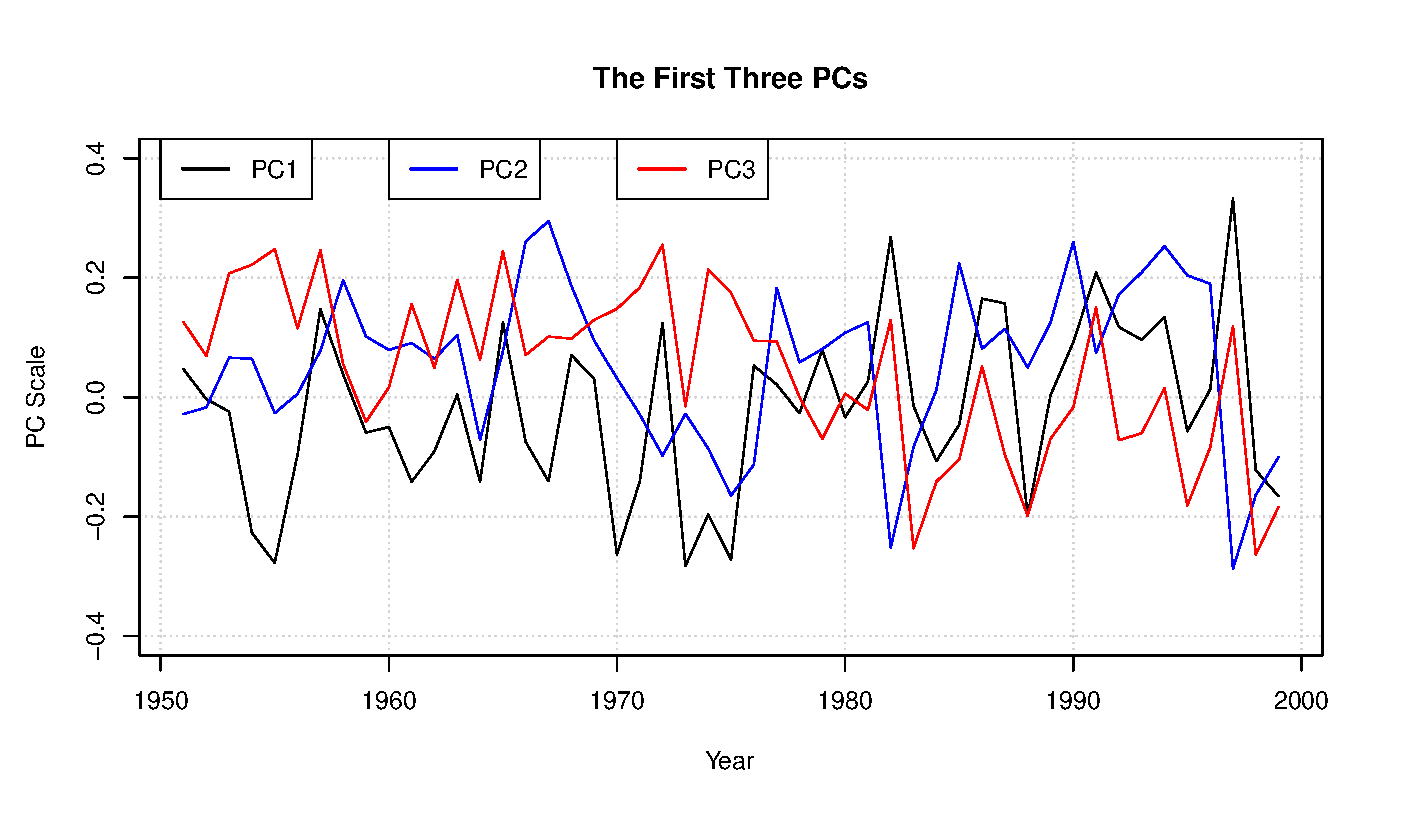
\includegraphics{Figures/Prob1/PC}
			
			\item  El Nino signals should show in the figures of Steps (b) and (c). Make a brief description of the El Ninos.
			\\ \\
			You can see from the EOF's and PC's that the temperature spikes in the same location and the same time in the pacific ocean consistently.  These spikes are consistent with the data that we have on the El Ninos.  The El Ninos spike in temperature in the pacific ocean at $200^\circ$ Latitude on the equator and around the summer time.  During these El Ninos as well, we can see that the wind reverses to become western winds instead of eastern winds.
			
		\end{enumerate}
		
	\end{problem}

	\begin{problem}{3-4 Exercise (5.9)}
		Make an SVD data representation analysis for the $5^\circ \times 5^\circ$ latitude-longitude gridded
		annual (July-June) precipitation field from 1951-2000 over the tropical Pacific: ($20^\circ S -20^\circ N, 160^\circ E -100^\circ W$). 
		\begin{enumerate}[label = (\alph*)]
			\item Perform the SVD analysis for the data. Print out the first 10 eigenvalues.
			\\ \\
			Notice the first 10 eigenvalues can be found by $\lambda_i = \frac{d_i^2}{t}$
			\begin{figure}[h!]
				\centering
				\begin{tabular}{|c|c|c|c|c|}
					\hline
					105.4814490 & 22.2559501 &  5.4832410 &  3.3866133 &  2.8810880 \\
					2.1684325 &  1.4404727 &  1.2810827 &  0.9563928 &  0.7468040 \\
					\hline
				\end{tabular}
			\end{figure} 
\begin{Shaded}
\begin{Highlighting}[]
\CommentTok{#Problem 3-4}

\KeywordTok{setwd}\NormalTok{(}\StringTok{'C:/Users/Stephen Giang/Documents/Math336Files'}\NormalTok{)}
\NormalTok{readData =}\StringTok{ }\KeywordTok{read.csv}\NormalTok{(}\StringTok{'PrcpRecon5degAnn.csv'}\NormalTok{)}

\NormalTok{pacific =}\StringTok{ }\KeywordTok{subset}\NormalTok{(readData, Lat }\OperatorTok{>=}\StringTok{ }\DecValTok{-20} \OperatorTok{&}\StringTok{ }\NormalTok{Lat }\OperatorTok{<=}\StringTok{ }\DecValTok{20}\NormalTok{)   }\CommentTok{#20S  - 20N}
\NormalTok{pacific =}\StringTok{ }\KeywordTok{subset}\NormalTok{(pacific, Lon }\OperatorTok{>=}\StringTok{ }\DecValTok{160} \OperatorTok{&}\StringTok{ }\NormalTok{Lon }\OperatorTok{<=}\StringTok{ }\DecValTok{260}\NormalTok{)  }\CommentTok{#160E - 100W}
\NormalTok{pacific =}\StringTok{ }\NormalTok{pacific[, }\DecValTok{54}\OperatorTok{:}\DecValTok{102}\NormalTok{] }\CommentTok{#1951 - 1999}

\NormalTok{yearDiff =}\StringTok{ }\DecValTok{1999} \OperatorTok{-}\StringTok{ }\DecValTok{1951} \OperatorTok{+}\StringTok{ }\DecValTok{1}
\NormalTok{svdPacific =}\StringTok{ }\KeywordTok{svd}\NormalTok{(pacific)}
\NormalTok{D =}\StringTok{ }\KeywordTok{diag}\NormalTok{(svdPacific}\OperatorTok{$}\NormalTok{d)}
\NormalTok{U =}\StringTok{ }\NormalTok{svdPacific}\OperatorTok{$}\NormalTok{u}
\NormalTok{V =}\StringTok{ }\NormalTok{svdPacific}\OperatorTok{$}\NormalTok{v}

\NormalTok{eigVals =}\StringTok{ }\NormalTok{(svdPacific}\OperatorTok{$}\NormalTok{d[}\DecValTok{1}\OperatorTok{:}\DecValTok{10}\NormalTok{])}\OperatorTok{^}\DecValTok{2} \OperatorTok{/}\StringTok{ }\NormalTok{yearDiff}
\NormalTok{eigVals}
\end{Highlighting}
\end{Shaded}

\begin{verbatim}
##  [1] 105.4814490  22.2559501   5.4832410   3.3866133   2.8810880   
##  [6]   2.1684325   1.4404727   1.2810827   0.9563928   0.7468040
\end{verbatim}
			\skipline
			\item  Plot the map of the first three U column vectors, which are the spatial patterns of the
			data field, and are also known as Empirical Orthogonal Functions (EOFs).
\begin{Shaded}
\begin{Highlighting}[]
\NormalTok{x =}\StringTok{ }\KeywordTok{seq}\NormalTok{(}\OperatorTok{-}\FloatTok{17.5}\NormalTok{, }\FloatTok{17.5}\NormalTok{, }\DataTypeTok{by=}\DecValTok{5}\NormalTok{)  }\CommentTok{# lat}
\NormalTok{y =}\StringTok{ }\KeywordTok{seq}\NormalTok{(}\FloatTok{162.5}\NormalTok{, }\FloatTok{257.5}\NormalTok{, }\DataTypeTok{by=}\DecValTok{5}\NormalTok{) }\CommentTok{# lon}
\NormalTok{numLatVals =}\StringTok{ }\KeywordTok{length}\NormalTok{(x)}
\NormalTok{numLonVals =}\StringTok{ }\KeywordTok{length}\NormalTok{(y)}
\NormalTok{time =}\StringTok{ }\DecValTok{1951} \OperatorTok{:}\StringTok{ }\DecValTok{1999}

\NormalTok{int=}\KeywordTok{seq}\NormalTok{(}\OperatorTok{-}\FloatTok{0.2}\NormalTok{,}\FloatTok{0.2}\NormalTok{,}\DataTypeTok{length.out=}\DecValTok{81}\NormalTok{)}
\NormalTok{rgb.palette=}\KeywordTok{colorRampPalette}\NormalTok{(}\KeywordTok{c}\NormalTok{(}\StringTok{'black'}\NormalTok{,}\StringTok{'blue'}\NormalTok{, }\StringTok{'darkgreen'}\NormalTok{,}
                               \StringTok{'green'}\NormalTok{, }\StringTok{'yellow'}\NormalTok{,}\StringTok{'pink'}\NormalTok{,}\StringTok{'red'}\NormalTok{,}\StringTok{'maroon'}\NormalTok{),}
                               \DataTypeTok{interpolate=}\StringTok{'spline'}\NormalTok{)}
\KeywordTok{suppressWarnings}\NormalTok{(}\KeywordTok{library}\NormalTok{(maps))}
\end{Highlighting}
\end{Shaded}
\newpage
\begin{Shaded}
\begin{Highlighting}[]
\NormalTok{umat =}\StringTok{ }\KeywordTok{matrix}\NormalTok{(U[,}\DecValTok{1}\NormalTok{], }\DataTypeTok{nrow =}\NormalTok{ numLonVals)}
\KeywordTok{filled.contour}\NormalTok{(y, x, umat, }\DataTypeTok{color.palette=}\NormalTok{rgb.palette, }\DataTypeTok{levels=}\NormalTok{int,}
               \DataTypeTok{xlim=}\KeywordTok{c}\NormalTok{(}\DecValTok{120}\NormalTok{,}\DecValTok{300}\NormalTok{),}\DataTypeTok{ylim=}\KeywordTok{c}\NormalTok{(}\OperatorTok{-}\DecValTok{40}\NormalTok{,}\DecValTok{40}\NormalTok{),}
               \DataTypeTok{plot.title=}\KeywordTok{title}\NormalTok{(}\DataTypeTok{main=}\StringTok{"EOF1 of the Tropical Pacific}
                                     \StringTok{ Precipitation Data"}\NormalTok{,}
                                \DataTypeTok{xlab=}\StringTok{"Latitude"}\NormalTok{,}\DataTypeTok{ylab=}\StringTok{"Longitude"}\NormalTok{),}
               \DataTypeTok{plot.axes=}\NormalTok{\{}\KeywordTok{axis}\NormalTok{(}\DecValTok{1}\NormalTok{); }\KeywordTok{axis}\NormalTok{(}\DecValTok{2}\NormalTok{); }\KeywordTok{map}\NormalTok{(}\StringTok{'world2'}\NormalTok{, }\DataTypeTok{add=}\OtherTok{TRUE}\NormalTok{); }\KeywordTok{grid}\NormalTok{()\},}
               \DataTypeTok{key.title=}\KeywordTok{title}\NormalTok{(}\DataTypeTok{main=}\StringTok{"[mm]"}\NormalTok{))}
\end{Highlighting}
\end{Shaded}
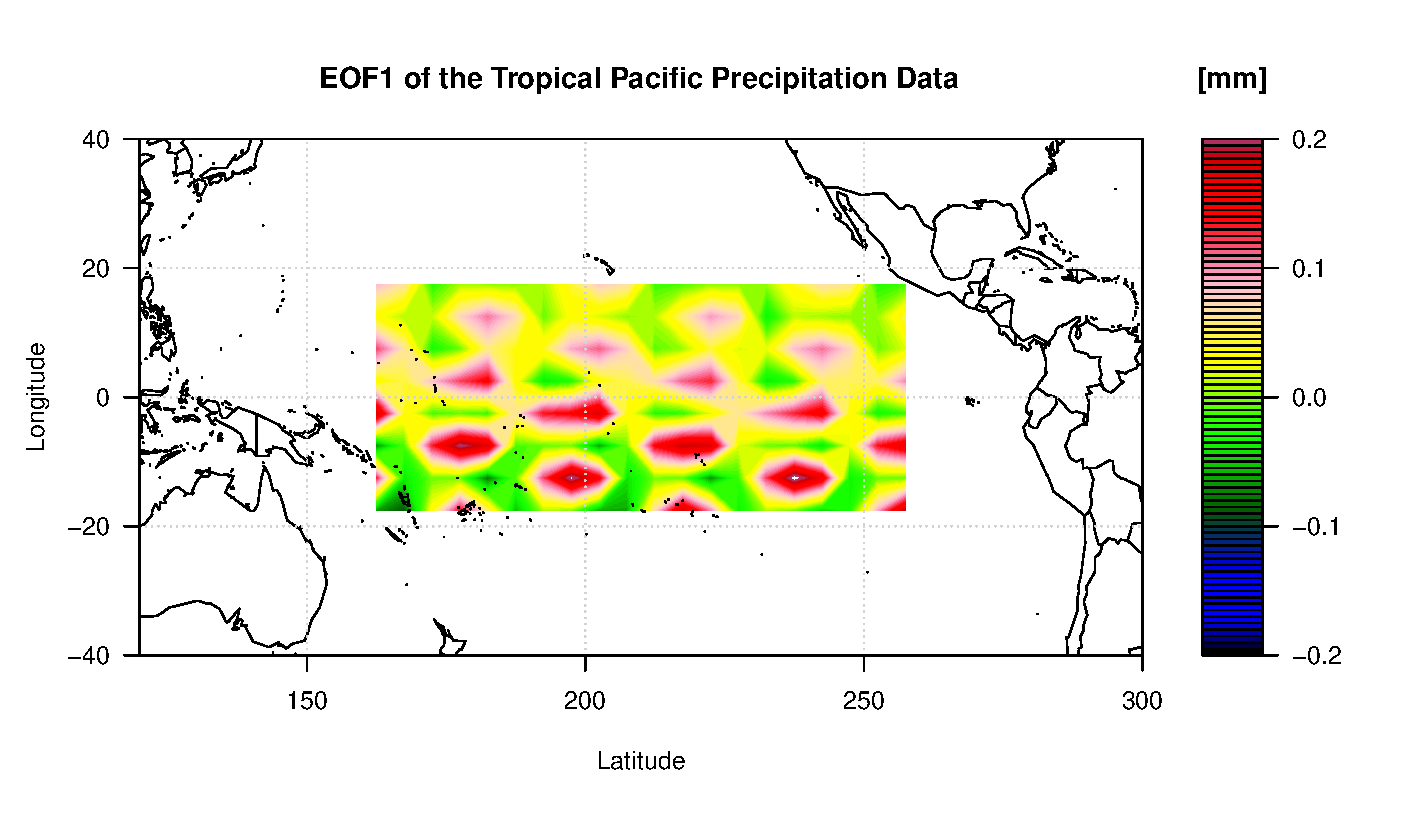
\includegraphics[height = 7cm]{Figures/Prob3/EOF1}
\begin{Shaded}
\begin{Highlighting}[]
\NormalTok{umat =}\StringTok{ }\KeywordTok{matrix}\NormalTok{(U[,}\DecValTok{2}\NormalTok{], }\DataTypeTok{nrow =}\NormalTok{ numLonVals)}
\KeywordTok{filled.contour}\NormalTok{(y, x, umat, }\DataTypeTok{color.palette=}\NormalTok{rgb.palette, }\DataTypeTok{levels=}\NormalTok{int,}
               \DataTypeTok{xlim=}\KeywordTok{c}\NormalTok{(}\DecValTok{120}\NormalTok{,}\DecValTok{300}\NormalTok{),}\DataTypeTok{ylim=}\KeywordTok{c}\NormalTok{(}\OperatorTok{-}\DecValTok{40}\NormalTok{,}\DecValTok{40}\NormalTok{),}
               \DataTypeTok{plot.title=}\KeywordTok{title}\NormalTok{(}\DataTypeTok{main=}\StringTok{"EOF2 of the Tropical Pacific}
                                     \StringTok{ Precipitation Data"}\NormalTok{,}
                                \DataTypeTok{xlab=}\StringTok{"Latitude"}\NormalTok{,}\DataTypeTok{ylab=}\StringTok{"Longitude"}\NormalTok{),}
               \DataTypeTok{plot.axes=}\NormalTok{\{}\KeywordTok{axis}\NormalTok{(}\DecValTok{1}\NormalTok{); }\KeywordTok{axis}\NormalTok{(}\DecValTok{2}\NormalTok{); }\KeywordTok{map}\NormalTok{(}\StringTok{'world2'}\NormalTok{, }\DataTypeTok{add=}\OtherTok{TRUE}\NormalTok{); }\KeywordTok{grid}\NormalTok{()\},}
               \DataTypeTok{key.title=}\KeywordTok{title}\NormalTok{(}\DataTypeTok{main=}\StringTok{"[mm]"}\NormalTok{))}
\end{Highlighting}
\end{Shaded}
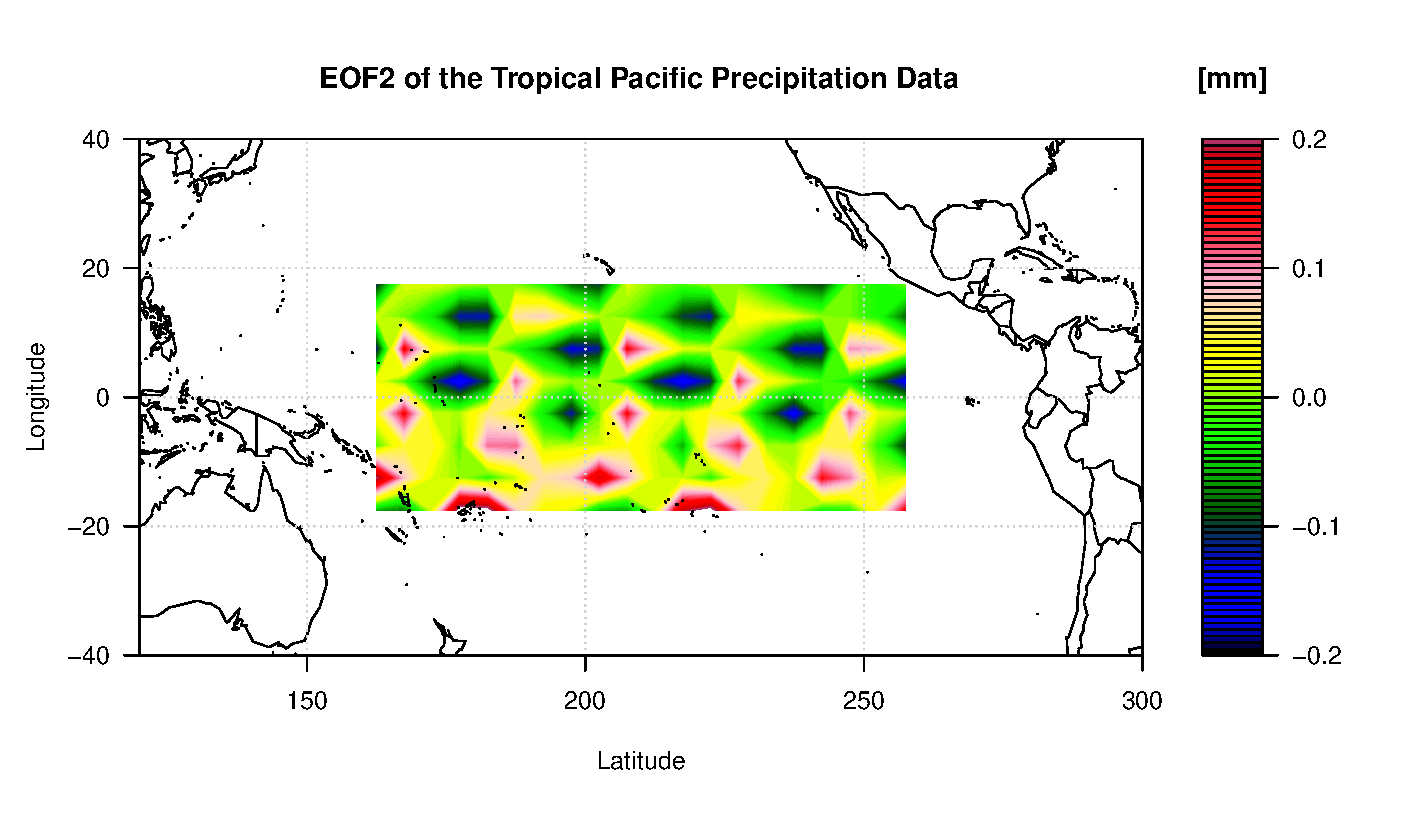
\includegraphics[height = 7cm]{Figures/Prob3/EOF2}
\begin{Shaded}
\begin{Highlighting}[]
\NormalTok{umat =}\StringTok{ }\KeywordTok{matrix}\NormalTok{(U[,}\DecValTok{3}\NormalTok{], }\DataTypeTok{nrow =}\NormalTok{ numLonVals)}
\KeywordTok{filled.contour}\NormalTok{(y, x, umat, }\DataTypeTok{color.palette=}\NormalTok{rgb.palette, }\DataTypeTok{levels=}\NormalTok{int,}
               \DataTypeTok{xlim=}\KeywordTok{c}\NormalTok{(}\DecValTok{120}\NormalTok{,}\DecValTok{300}\NormalTok{),}\DataTypeTok{ylim=}\KeywordTok{c}\NormalTok{(}\OperatorTok{-}\DecValTok{40}\NormalTok{,}\DecValTok{40}\NormalTok{),}
               \DataTypeTok{plot.title=}\KeywordTok{title}\NormalTok{(}\DataTypeTok{main=}\StringTok{"EOF3 of the Tropical Pacific}
                                     \StringTok{ Precipitation Data"}\NormalTok{,}
                                \DataTypeTok{xlab=}\StringTok{"Latitude"}\NormalTok{,}\DataTypeTok{ylab=}\StringTok{"Longitude"}\NormalTok{),}
               \DataTypeTok{plot.axes=}\NormalTok{\{}\KeywordTok{axis}\NormalTok{(}\DecValTok{1}\NormalTok{); }\KeywordTok{axis}\NormalTok{(}\DecValTok{2}\NormalTok{); }\KeywordTok{map}\NormalTok{(}\StringTok{'world2'}\NormalTok{, }\DataTypeTok{add=}\OtherTok{TRUE}\NormalTok{); }\KeywordTok{grid}\NormalTok{()\},}
               \DataTypeTok{key.title=}\KeywordTok{title}\NormalTok{(}\DataTypeTok{main=}\StringTok{"[mm]"}\NormalTok{))}
\end{Highlighting}
\end{Shaded}
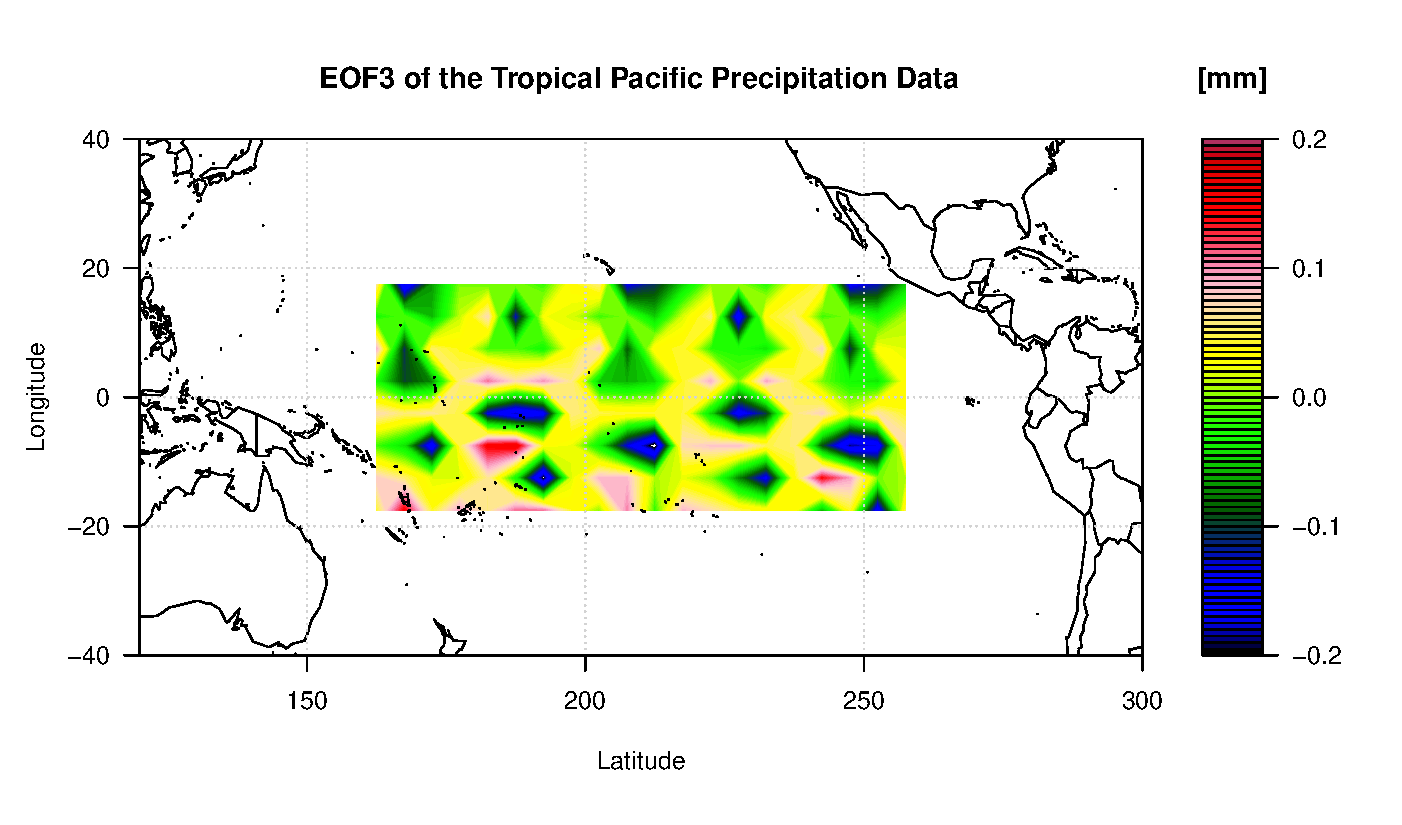
\includegraphics[height = 8cm]{Figures/Prob3/EOF3}
\newpage
			\item Plot the time series of the first three V column vectors, which are the temporal patterns
			of the data field, and are also known as Principal Components (PCs).

			\skipline
\begin{Shaded}
\begin{Highlighting}[]
\KeywordTok{plot}\NormalTok{(time, V[,}\DecValTok{1}\NormalTok{], }\StringTok{'l'}\NormalTok{, }\DataTypeTok{col =} \StringTok{'black'}\NormalTok{,}
     \DataTypeTok{xlab =} \StringTok{'Year'}\NormalTok{, }\DataTypeTok{ylab =} \StringTok{'PC Scale'}\NormalTok{, }\DataTypeTok{ylim=}\KeywordTok{c}\NormalTok{(}\OperatorTok{-}\FloatTok{0.8}\NormalTok{,}\FloatTok{0.4}\NormalTok{), }
     \DataTypeTok{main =} \StringTok{'The First Three PCs'}\NormalTok{, }\DataTypeTok{panel.first=}\KeywordTok{grid}\NormalTok{())}
\KeywordTok{lines}\NormalTok{(time, V[,}\DecValTok{2}\NormalTok{], }\DataTypeTok{type=}\StringTok{"l"}\NormalTok{, }\DataTypeTok{col=}\StringTok{"blue"}\NormalTok{)}
\KeywordTok{lines}\NormalTok{(time, V[,}\DecValTok{3}\NormalTok{], }\DataTypeTok{type=}\StringTok{"l"}\NormalTok{, }\DataTypeTok{col=}\StringTok{"red"}\NormalTok{)}


\KeywordTok{legend}\NormalTok{(}\DecValTok{1950}\NormalTok{,}\FloatTok{0.448}\NormalTok{, }\StringTok{'PC1'}\NormalTok{,}\DataTypeTok{lwd=}\DecValTok{2}\NormalTok{ )}
\KeywordTok{legend}\NormalTok{(}\DecValTok{1960}\NormalTok{,}\FloatTok{0.448}\NormalTok{, }\StringTok{'PC2'}\NormalTok{,}\DataTypeTok{lwd=}\DecValTok{2}\NormalTok{, }\DataTypeTok{col=}\StringTok{"blue"}\NormalTok{)}
\KeywordTok{legend}\NormalTok{(}\DecValTok{1970}\NormalTok{,}\FloatTok{0.448}\NormalTok{, }\StringTok{'PC3'}\NormalTok{,}\DataTypeTok{lwd=}\DecValTok{2}\NormalTok{, }\DataTypeTok{col=}\StringTok{"red"}\NormalTok{)}
\end{Highlighting}
\end{Shaded}
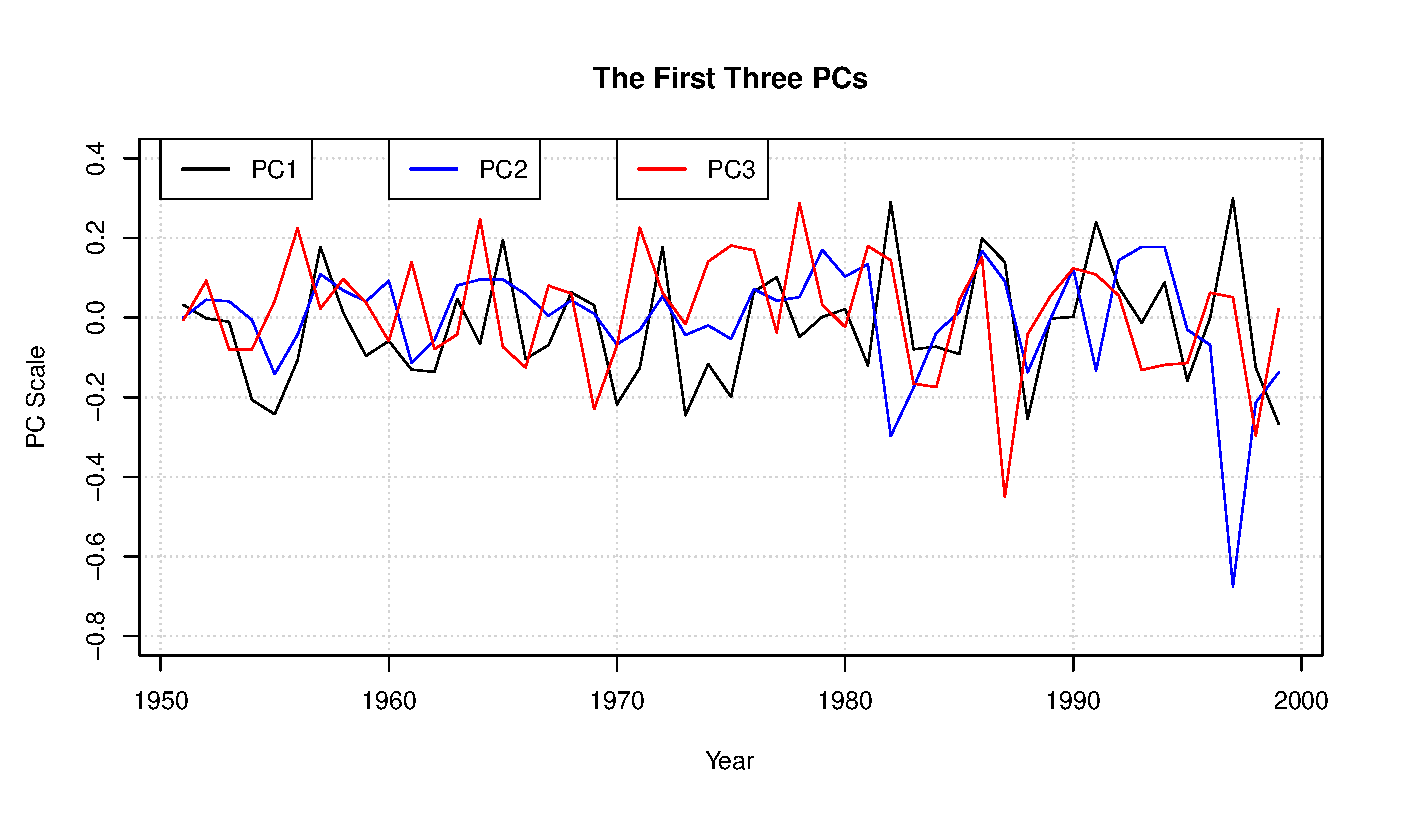
\includegraphics{Figures/Prob3/PC}
			\item El Nino signals should show in the figures of Steps (b) and (c). Compare the El Nino
			signals from the precipitation data with those from the temperature data. Use 100-200
			words to describe your comparison.
			\\ \\
			We can see from this that where the temperature is lower, we can see higher amounts of precipitation.  This is because of the El Nino signals show a change in winds that will lead to a change in temperature and precipitation. From the PC's we can see that the precipitation dropped a fairly large amount within the decade of 1990 - 2000. 
		\end{enumerate}
	\end{problem}

	\begin{problem}{5 Exercise (6.1)}
		Suppose that the greenhouse effect results in a net energy gain of the Earth’s surface
		by 1.0 [$Wm^{-2}$]. If the gained heat is all used to heat the Earth’s atmosphere, how many years will be needed to warm the Earth’s entire atmosphere by $1.0^\circ$C? If the heat is all used to heat the Earth’s surface water, including the water in the oceans, lakes, and rivers, how many years will it take to warm the water by $1.0^\circ$C? Make comments about this study’s
		implications for global warming.
		\\ \\
		\textit{Hint: You can find the relevant information about the Earth’s atmosphere and water in
		this book or from the Internet}
		\\ \\
		Source: \url{https://atmos.washington.edu/~dennis/321/321_Lecture_12.pdf}
		\\ \\
		Notice the following for heating the Earth's Atmosphere by $1^\circ$ C or by 1 K.  
		\\ \\
		We can use the following equation to determine the mass of the Earth's Atmosphere and Water per square meter:
		\[F = ma \qquad \rightarrow \qquad P_s = mg \]
		where $P_s$ is the pressure at sea level and $g$ is the acceleration of gravity. 
		\\ \\
		From here notice the following:
		\[P_s = 101,325 Pa = 101,325 \frac{kg}{m s^2} = m \left(9.81\frac{m}{s^2}\right) \qquad \rightarrow \qquad m = 10,328.7462 \frac{kg}{m^2}\]
		Now, we can determine the time to heat up the Earth's atmosphere or the Earth's water by $1^\circ$C using the following equation:
		\begin{align*}
			q = 1\,\frac{W}{m^2} = 1\,\frac{J}{s\,m^2} = mc\Delta T = \left(10,328.7462\,\frac{kg}{m^2} \right)c\Delta T 
		\end{align*}
		where $c$ is the specific heat capacity of the desired item.
		\\ \\ \\
		We get the following for the \textbf{Earth's Atmosphere} with $c = 1003.5 \frac{J}{kg\,K}$:
		\[\Delta T = \frac{q}{mc} = \frac{1\,\frac{J}{s\,m^2}}{\left(10,328.7462\,\frac{kg}{m^2} \right)\left( 1003.5 \frac{J}{kg\,K}\right)} \frac{K}{s} \left(\frac{31,536,000\,s}{yr}\right) = 3.042577 \frac{K}{yr}\]
		With this, we can see that:
		\[3.042577\,\frac{K}{yr} = 3.042577\,\frac{^\circ C}{yr} = 0.3286687\,\frac{yr}{^\circ C} = \boldsymbol{120\,\frac{days}{1^\circ C}}\]
		\\ \\
		We get the following for the \textbf{Earth's Water} with $c = 4184 \frac{J}{kg\,K}$:
		\[\Delta T = \frac{q}{mc} = \frac{1\,\frac{J}{s\,m^2}}{\left(10,328.7462\,\frac{kg}{m^2} \right)\left( 4184 \frac{J}{kg\,K}\right)} \frac{K}{s} \left(\frac{31,536,000\,s}{yr}\right) = 0.729739 \frac{K}{yr}\]
		With this, we can see that:
		\[0.729739\,\frac{K}{yr} = 0.729739\,\frac{^\circ C}{yr} = \boldsymbol{1.370353\,\frac{yr}{^\circ C}}\]
	\end{problem}

	\begin{problem}{6 Exercise (6.5)}
		Repeat Elisha Mitchell’s calculation with the current data you can find online, such
		as the North Carolina Climate Office NC ECONet, and make your own estimation of the
		elevation of Mount Mitchell using the hypsometric equation.
		\\ \\
		Information Taken on: Sunday, November 22, 2020 @ 8:35PM EST.
		\\ \\
		Station BURN (Base): Burnsville Tower Station: Location ($35.91892^\circ$ N, $82.26035^\circ$ W ), Elevation (2702 ft above Sea Level), Temperature ($9.4^\circ$ C), Pressure (924.9 mb) 
		\\ \\
		Station MITC (Top): Mount Mitchell State Park Station: Location ($35.7585^\circ$ N, $82.2712^\circ$ W ), Elevation (6200 ft above Sea Level), Temperature ($4.5^\circ$ C), Pressure (811.8 mb).
		\begin{align*}
			z_2 &= z_1 + \frac{2RT_1T_2}{g(T_1 + T_2)}\ln\left(\frac{p_1}{p_2}\right) \\
			&= (2702)(0.3408) + \frac{2(287.055)(273.15 + 9.4)(273.15 + 4.5)}{9.80665(273.15 + 9.4 + 273.15 + 4.5)}\ln\left(\frac{924.9}{811.8}\right) \\
			&= 1990.160413\,m \\
			&= 5839.672572\,ft
		\end{align*}
		This is about a 5\% error from the actual 6200ft elevation.  This is could be from the high humidity (95\%) or the high winds (20 mph).
	\end{problem}

	\begin{problem}{7 Exercise (6.6)}
		Calculate the elevation of a high mountain peak near your location, or in another place with which you are familiar, using observed data and the hypsometric equation.
		\\ \\
		Information Taken on: Saturday, November 28, 2020 @ 3:33 PM \& @4:18 PM
		\\ \\
		Mount Woodson (Base): Elevation (1588 ft above Sea Level), Temperature ($16^\circ$ C), Pressure (958.5 mb) 
		\\ \\
		Mount Woodson (Top): Elevation (2402 ft above Sea Level), Temperature ($16^\circ$ C), Pressure (919.5 mb).
		\begin{align*}
			z_2 &= z_1 + \frac{2RT_1T_2}{g(T_1 + T_2)}\ln\left(\frac{p_1}{p_2}\right) \\
			&= (1588)(0.3408) + \frac{2(287.055)(273.15 + 16)(273.15 + 16)}{9.80665(273.15 + 16 + 273.15 + 16)}\ln\left(\frac{958.5}{919.5}\right) \\
			&= 892.7743933\,m \\
			&= 2619.643173\,ft
		\end{align*}
		This is about a 9\% error from the actual 2402ft elevation.  This is most likely to be from an inaccurate barometer reading from a weak GPS signal.  When reading online, it says that this mountain has a peak of between 2500 ft - 2800 ft depending on different sources, so our calculation is not too far off.
		\\ \\
		For this problem, I was unable to find accurate barometer readings of these local mountains online due to the fact they weren't major mountains in the US.  So I decided to hike this mountain, and calculate the barometric pressure, temperature, and altitude using my phones GPS.  Below, you'll see the data collected. 
		\\
		\begin{figure}[h!]
			\centering
			\begin{subfigure}{.4\textwidth}
				\centering
				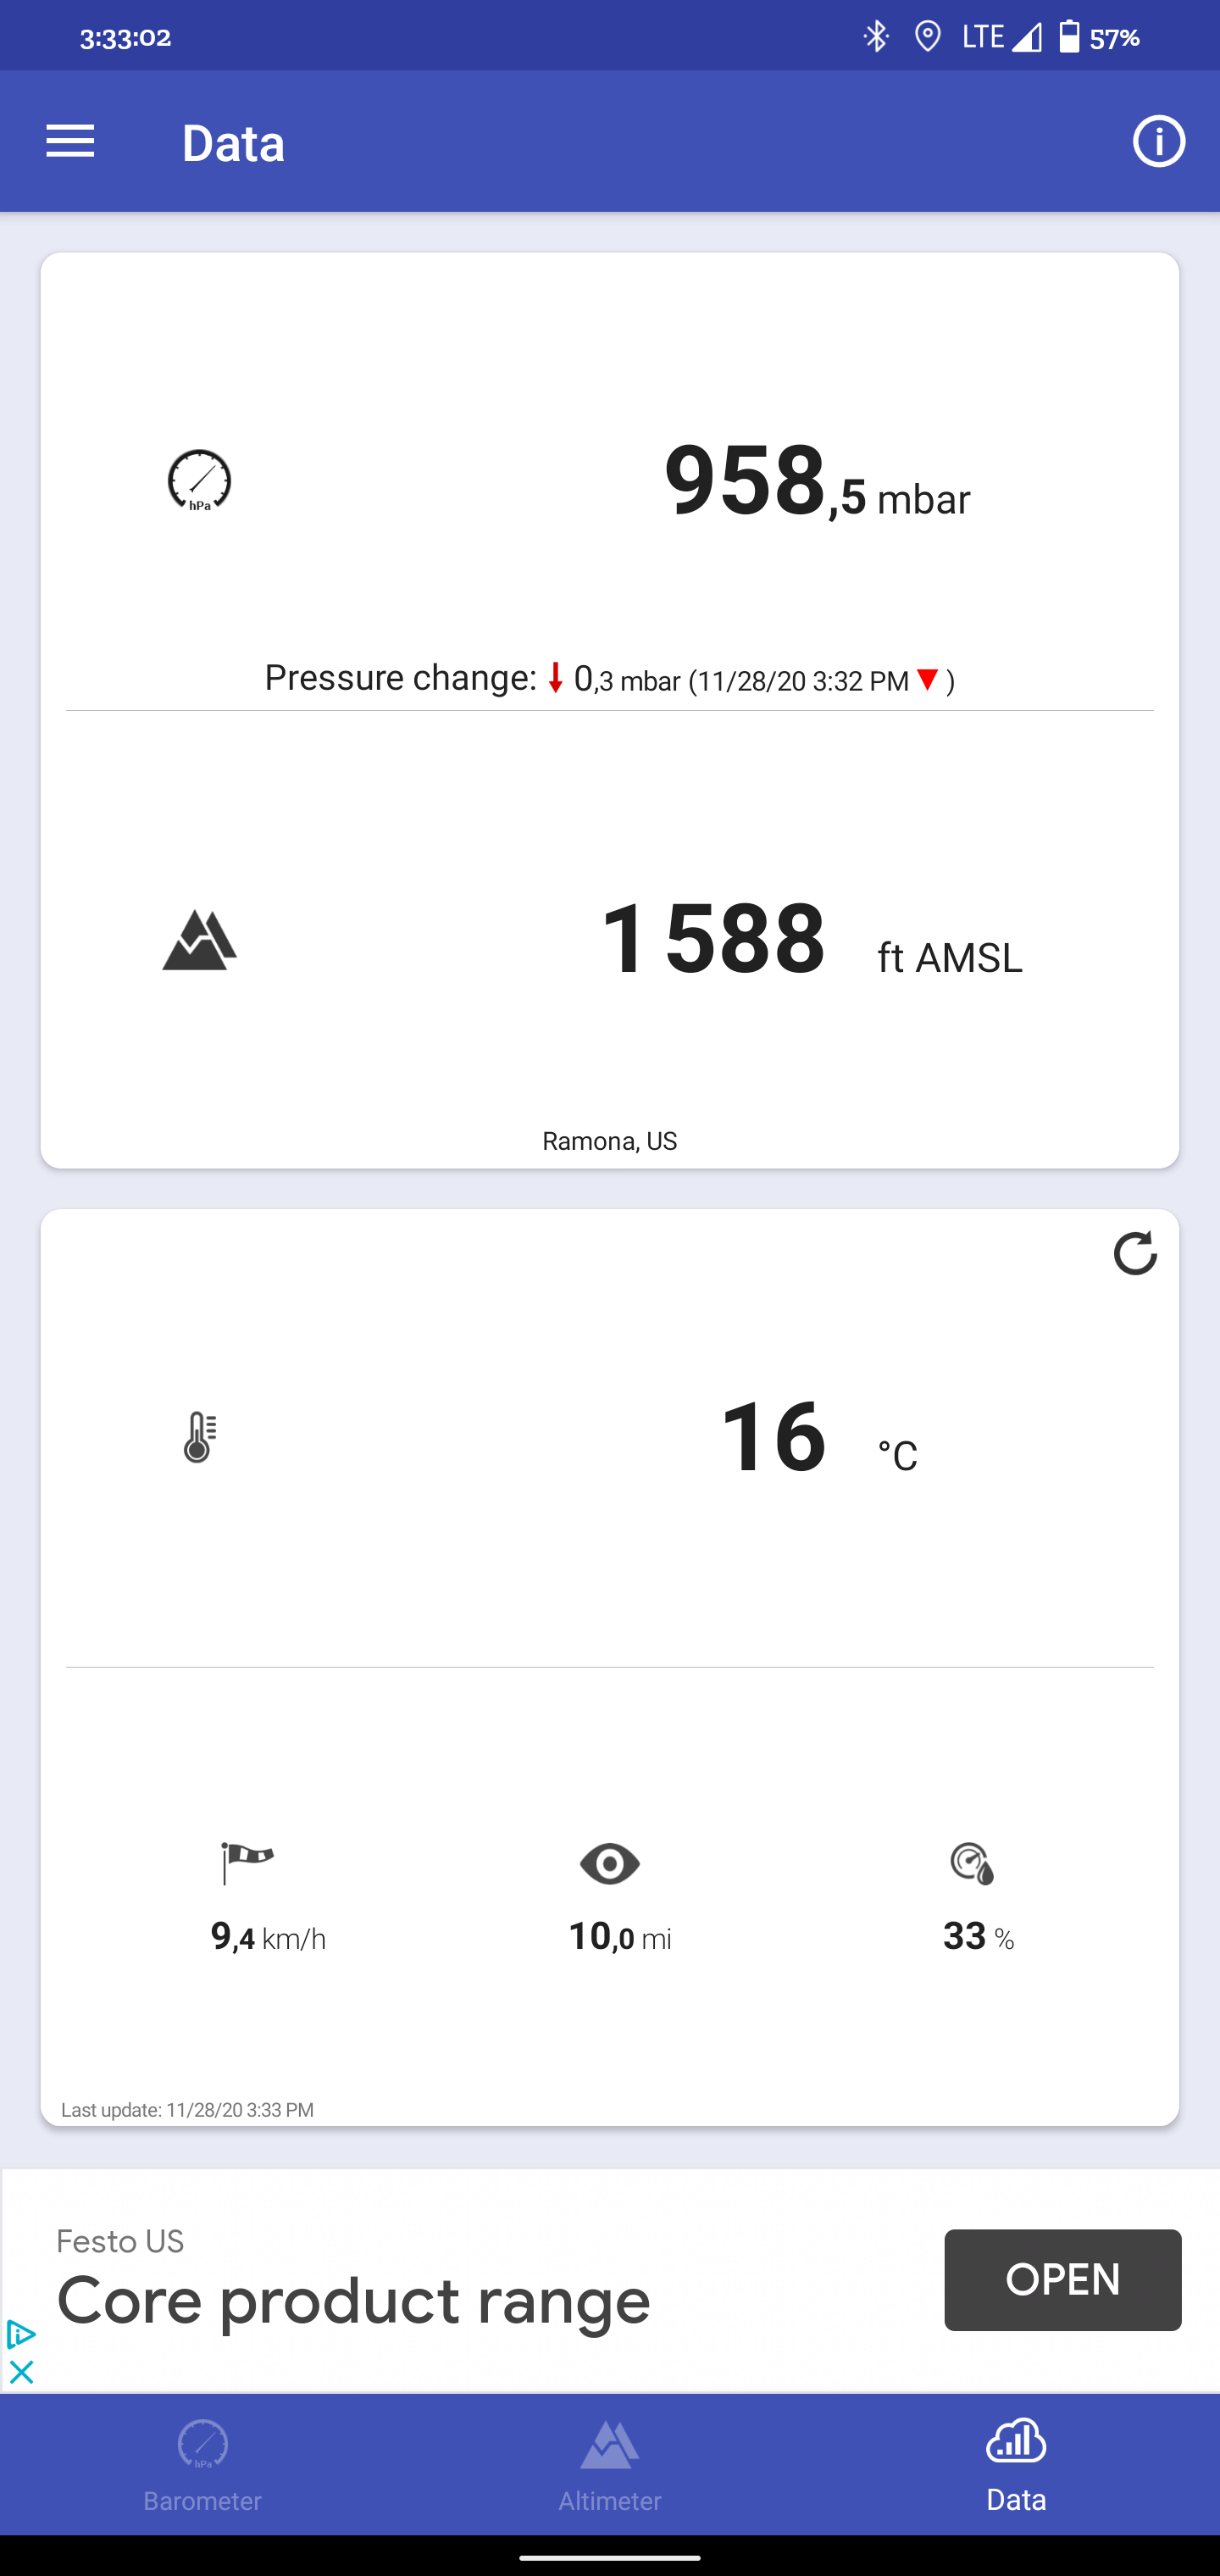
\includegraphics[height = 9cm]{Figures/Prob7/Base.png}
			\end{subfigure}
			\begin{subfigure}{.4\textwidth}
				\centering
				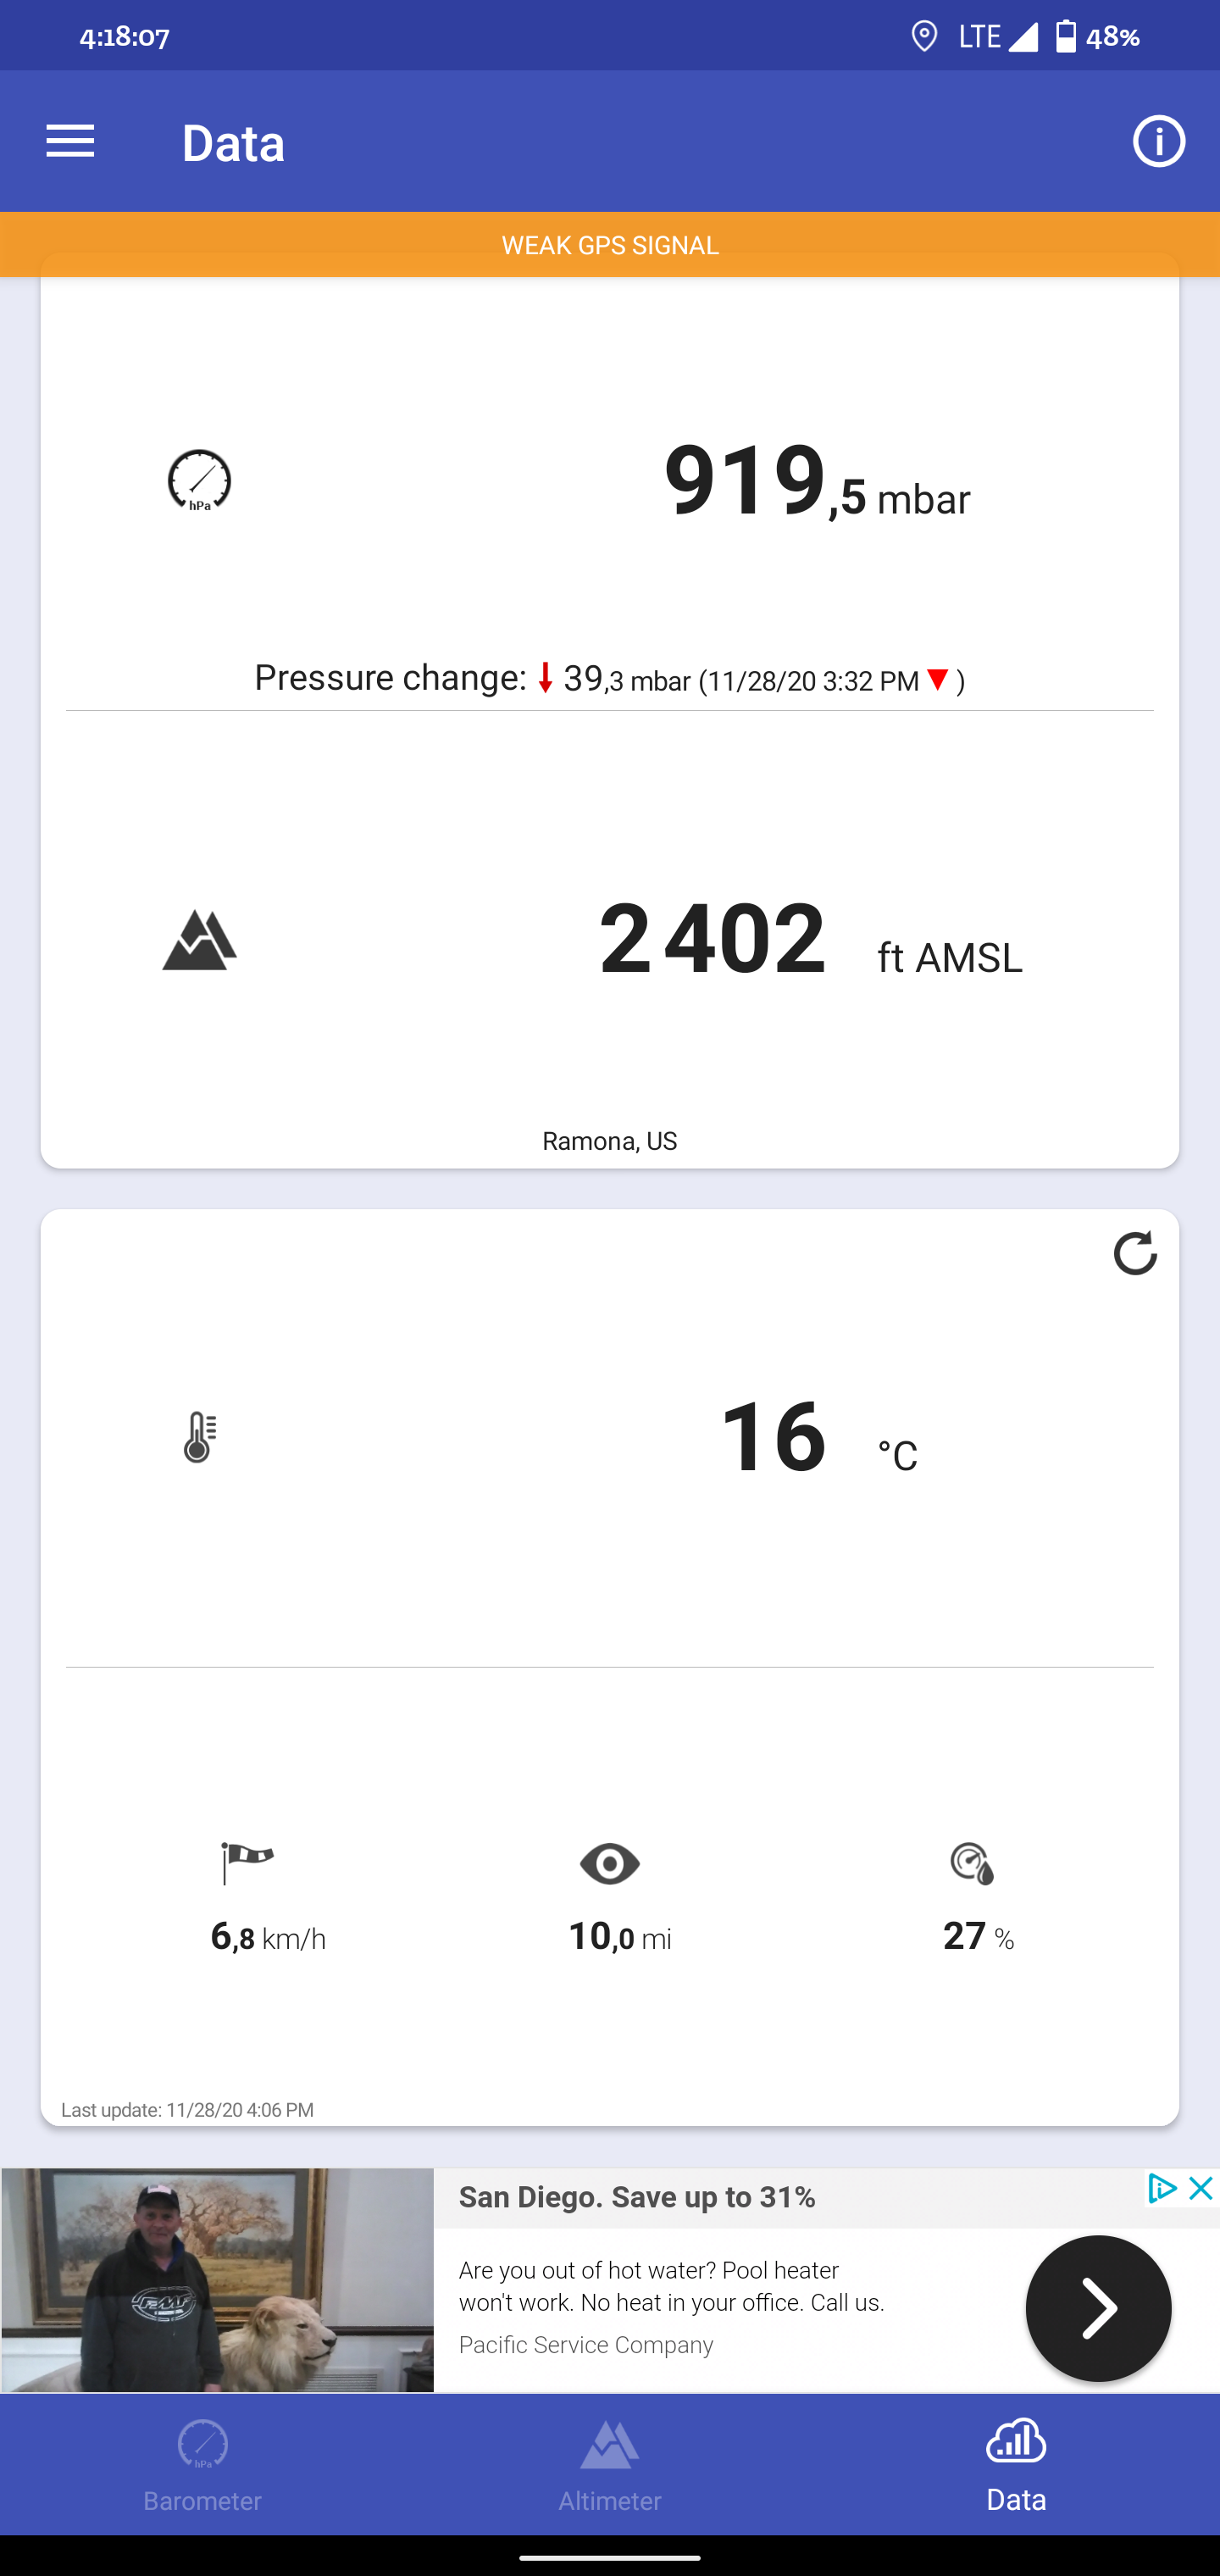
\includegraphics[height = 9cm]{Figures/Prob7/Top.png}
			\end{subfigure}
		\end{figure}
	\end{problem}

	\begin{problem}{8}
		\begin{enumerate}[label = (\alph*)]
			\item Derive the Buffon's needle problem solution when the needle length is longer than the gap of two lines.
			\\ \\
			Notice the following:
			\\ \\
			Let $y$ be position of the lower end of the needle, $d$ be the gap between the two lines, and $\ell > d$ be the length of the needle.
			\\ \\
			We have the probability region be in the space $[-\pi/2, \pi/2] \times [0,d]$.  Thus we get the probability region is $A = \pi d$.
			\\ \\
			We can use the following equation to determine the angles for which the line will cross the top line:
			\[y + \ell \cos \alpha \geq d\]
			The lower bound, $y = 0$, means that the only way for the needle to cross the top line is if at least $\ell \cos \alpha = d$.  From this we can see that this is the case for:
			\[\alpha = \arccos \frac{d}{l}\]
			Using trig rules, we can see that the line definitely crosses for $\theta \in [-\alpha, \alpha]$.  From this we get the following "definite" area 
			\[A_x = 2\alpha d\]
			Now for the indefinite area, we can find this by taking the following integral:
			\[A_c = 2\int_{\alpha}^{\pi/2} \left[d - (d - \ell \cos \theta)\right]\,d\theta = 2\ell \int_{\alpha}^{\pi/2} \cos \theta \,d\theta = 2\ell - 2\ell \sin \alpha\] 
			Using algebra, we see the following inequality:
			\[\ell \sin \alpha = \sqrt{\ell^2 - d^2}\]
			Now from here, we get the probability of a needle crossing the top line being the following:
			\begin{align*}
				P_L = \frac{A_x + A_c}{A} &= \frac{1}{\pi d}\left[2\alpha d + 2\ell - 2\ell \sin \alpha \right] \\
				&= \frac{2}{\pi d}\left[\alpha d + \ell - \sqrt{\ell^2 - d^2}\right] \\
				&= \frac{2}{\pi }\left[\alpha + \frac{\ell}{d} - \sqrt{\left(\frac{\ell}{d}\right)^2 - 1}\right] \\
				&= \frac{2}{\pi }\left[\arccos\left(\frac{d}{\ell}\right) + \frac{\ell}{d} - \sqrt{\left(\frac{\ell}{d}\right)^2 - 1}\right]
			\end{align*}
			\newpage
			\item Write an R program to simulate the above Buffon's needle problem in (a). \\
\begin{Shaded}
\begin{Highlighting}[]
\CommentTok{# Problem 8}

\NormalTok{BuffonLongSim =}\StringTok{ }\ControlFlowTok{function}\NormalTok{(d, l, }\DataTypeTok{n =} \DecValTok{10000}\NormalTok{) \{}
\NormalTok{  k =}\StringTok{ }\DecValTok{0}
  \ControlFlowTok{for}\NormalTok{ (i }\ControlFlowTok{in} \DecValTok{1} \OperatorTok{:}\StringTok{ }\NormalTok{n) \{}
\NormalTok{    y =}\StringTok{ }\KeywordTok{runif}\NormalTok{(}\DecValTok{1}\NormalTok{, }\DataTypeTok{min =} \DecValTok{0}\NormalTok{, }\DataTypeTok{max =}\NormalTok{ d)}
\NormalTok{    theta =}\StringTok{ }\KeywordTok{runif}\NormalTok{(}\DecValTok{1}\NormalTok{, }\DataTypeTok{min =} \OperatorTok{-}\NormalTok{pi }\OperatorTok{/}\DecValTok{2}\NormalTok{, }\DataTypeTok{max =}\NormalTok{ pi}\OperatorTok{/}\DecValTok{2}\NormalTok{)}
    \ControlFlowTok{if}\NormalTok{ (y }\OperatorTok{+}\StringTok{ }\NormalTok{l}\OperatorTok{*}\KeywordTok{cos}\NormalTok{(theta) }\OperatorTok{>=}\StringTok{ }\NormalTok{d) \{}
\NormalTok{      k =}\StringTok{ }\NormalTok{k }\OperatorTok{+}\StringTok{ }\DecValTok{1}
\NormalTok{    \}}
\NormalTok{  \}}
\KeywordTok{return}\NormalTok{(k }\OperatorTok{/}\StringTok{ }\NormalTok{n)}
\NormalTok{\}}

\NormalTok{BuffonLongExact =}\StringTok{ }\ControlFlowTok{function}\NormalTok{(d, l) \{}
\NormalTok{  dl =}\StringTok{ }\NormalTok{d}\OperatorTok{/}\StringTok{ }\NormalTok{l}
\NormalTok{  ld =}\StringTok{ }\NormalTok{l }\OperatorTok{/}\StringTok{ }\NormalTok{d}
\NormalTok{  twopi =}\StringTok{ }\DecValTok{2} \OperatorTok{/}\StringTok{ }\NormalTok{pi}
  \KeywordTok{return}\NormalTok{( twopi }\OperatorTok{*}\StringTok{ }\NormalTok{( }\KeywordTok{acos}\NormalTok{(dl) }\OperatorTok{+}\StringTok{ }\NormalTok{ld }\OperatorTok{-}\StringTok{ }\KeywordTok{sqrt}\NormalTok{( (ld)}\OperatorTok{^}\DecValTok{2} \OperatorTok{-}\StringTok{ }\DecValTok{1}\NormalTok{) ) )}
\NormalTok{\}}
\end{Highlighting}
\end{Shaded}
\skipline
\begin{Shaded}
\begin{Highlighting}[]
\NormalTok{d =}\StringTok{ }\KeywordTok{floor}\NormalTok{(}\KeywordTok{runif}\NormalTok{(}\DecValTok{1}\NormalTok{, }\DataTypeTok{min =} \DecValTok{1}\NormalTok{, }\DataTypeTok{max =} \DecValTok{100}\NormalTok{))}
\NormalTok{l =}\StringTok{ }\KeywordTok{floor}\NormalTok{(}\KeywordTok{runif}\NormalTok{(}\DecValTok{1}\NormalTok{, }\DataTypeTok{min =} \DecValTok{1}\NormalTok{, }\DataTypeTok{max =} \DecValTok{100}\NormalTok{)) }\OperatorTok{+}\StringTok{ }\NormalTok{d   }\CommentTok{# l > d}
\end{Highlighting}
\end{Shaded}
\begin{Shaded}
\begin{Highlighting}[]
\KeywordTok{BuffonLongSim}\NormalTok{(d, l, }\DecValTok{10000}\NormalTok{)} \CommentTok{# d = 28, l = 81}
\end{Highlighting}
\end{Shaded}

\begin{verbatim}
## [1] 0.8899
\end{verbatim}

\begin{Shaded}
\begin{Highlighting}[]
\KeywordTok{BuffonLongExact}\NormalTok{(d, l)} \CommentTok{# d = 28, l = 81}
\end{Highlighting}
\end{Shaded}

\begin{verbatim}
## [1] 0.8888297
\end{verbatim}
		\end{enumerate}
	\end{problem}

	\begin{problem}{9}
		Write an R code for Monte Carlo simulation to calculate the volume of a unit ball in 8-dimensional space.
		\\ \\
\begin{Shaded}
\begin{Highlighting}[]
\CommentTok{# Problem 9}

\NormalTok{MCSim =}\StringTok{ }\ControlFlowTok{function}\NormalTok{(dim, }\DataTypeTok{n =} \DecValTok{10000}\NormalTok{) \{}
\NormalTok{  x =}\StringTok{ }\KeywordTok{matrix}\NormalTok{(}\KeywordTok{runif}\NormalTok{(dim}\OperatorTok{*}\NormalTok{n, }\DataTypeTok{min=} \DecValTok{-1}\NormalTok{, }\DataTypeTok{max =} \DecValTok{1}\NormalTok{), }\DataTypeTok{ncol =}\NormalTok{ dim)}
\NormalTok{  k =}\StringTok{ }\DecValTok{0}
  \ControlFlowTok{for}\NormalTok{ (i }\ControlFlowTok{in} \DecValTok{1} \OperatorTok{:}\StringTok{ }\NormalTok{n) \{}
    \ControlFlowTok{if}\NormalTok{ ( (}\KeywordTok{t}\NormalTok{(x[i,]) }\OperatorTok\StringTok{ }\NormalTok{x[i,]) }\OperatorTok{<}\StringTok{ }\DecValTok{1}\NormalTok{) \{}
\NormalTok{      k =}\StringTok{ }\NormalTok{k }\OperatorTok{+}\StringTok{ }\DecValTok{1}
\NormalTok{    \}}
\NormalTok{  \}}
  \KeywordTok{return}\NormalTok{( (k}\OperatorTok{/}\NormalTok{n) }\OperatorTok{*}\StringTok{ }\DecValTok{2}\OperatorTok{^}\NormalTok{dim )}
\NormalTok{\}}

\NormalTok{MCExact =}\StringTok{ }\ControlFlowTok{function}\NormalTok{(n,}\DataTypeTok{R=}\DecValTok{1}\NormalTok{) \{}
\NormalTok{  numer =}\StringTok{ }\NormalTok{pi}\OperatorTok{^}\NormalTok{(n}\OperatorTok{/}\DecValTok{2}\NormalTok{)}
\NormalTok{  denom =}\StringTok{ }\KeywordTok{gamma}\NormalTok{((n}\OperatorTok{/}\DecValTok{2}\NormalTok{) }\OperatorTok{+}\StringTok{ }\DecValTok{1}\NormalTok{)}
  \KeywordTok{return}\NormalTok{((numer}\OperatorTok{/}\NormalTok{denom)}\OperatorTok{*}\NormalTok{(R}\OperatorTok{^}\NormalTok{n))}
\NormalTok{\}}
\end{Highlighting}
\end{Shaded}
\skipline
\begin{Shaded}
\begin{Highlighting}[]
\KeywordTok{MCSim}\NormalTok{(}\DecValTok{8}\NormalTok{, }\DecValTok{100000}\NormalTok{)}
\end{Highlighting}
\end{Shaded}

\begin{verbatim}
## [1] 4.06016
\end{verbatim}

\begin{Shaded}
\begin{Highlighting}[]
\KeywordTok{MCExact}\NormalTok{(}\DecValTok{8}\NormalTok{)}
\end{Highlighting}
\end{Shaded}

\begin{verbatim}
## [1] 4.058712
\end{verbatim}
	
	\end{problem}

	\begin{problem}{10}
		When one roll two dice randomly, it is known that the event of two dice’s sum equal to 7 has a probability 1/6. Write an R code to simulate this process and verify this result.
		\\ \\
		We can verify this result through the following:
		\\ \\
		Each dice has numbers ranging from 1 - 6.  With this, each roll each dice has a chance of falling on 6 numbers.  This means there will be a total of $6^2 = 36$ combinations that 2 dice can be rolled.  Notice the numbers that add up to 7:
		\[(1 + 6), (2 + 5), (3 + 4), (4 + 3), (5 + 2), (6 + 1)\]
		Thus we get there is a $6/36 = 1/6$ probability of getting two dice whose sum at up to 7.
		\\ \\
		Notice the code below, that simulates a dice roll: \\
\begin{Shaded}
\begin{Highlighting}[]
\CommentTok{# Problem 10}

\NormalTok{diceRollSim =}\StringTok{ }\ControlFlowTok{function}\NormalTok{ (n) \{}
\NormalTok{  k =}\StringTok{ }\DecValTok{0}
  \ControlFlowTok{for}\NormalTok{ (i }\ControlFlowTok{in} \DecValTok{1} \OperatorTok{:}\StringTok{ }\NormalTok{n) \{}
\NormalTok{    a =}\StringTok{ }\KeywordTok{floor}\NormalTok{(}\KeywordTok{runif}\NormalTok{(}\DecValTok{1}\NormalTok{, }\DataTypeTok{min =} \DecValTok{1}\NormalTok{, }\DataTypeTok{max =} \DecValTok{6}\NormalTok{))}
\NormalTok{    b =}\StringTok{ }\KeywordTok{floor}\NormalTok{(}\KeywordTok{runif}\NormalTok{(}\DecValTok{1}\NormalTok{, }\DataTypeTok{min =} \DecValTok{1}\NormalTok{, }\DataTypeTok{max =} \DecValTok{6}\NormalTok{))}
  \ControlFlowTok{if}\NormalTok{ (a }\OperatorTok{+}\StringTok{ }\NormalTok{b }\OperatorTok{==}\StringTok{ }\DecValTok{7}\NormalTok{) \{}
\NormalTok{      k =}\StringTok{ }\NormalTok{k }\OperatorTok{+}\StringTok{ }\DecValTok{1}
\NormalTok{    \}}
\NormalTok{  \}}
  \KeywordTok{return}\NormalTok{(k }\OperatorTok{/}\StringTok{ }\NormalTok{n)}
\NormalTok{\}}

\NormalTok{diceRollExact =}\StringTok{ }\ControlFlowTok{function}\NormalTok{ () \{}
\NormalTok{  k =}\StringTok{ }\DecValTok{0}
  \ControlFlowTok{for}\NormalTok{ (i }\ControlFlowTok{in} \DecValTok{1} \OperatorTok{:}\StringTok{ }\DecValTok{6}\NormalTok{) \{}
    \ControlFlowTok{for}\NormalTok{ (j }\ControlFlowTok{in} \DecValTok{1} \OperatorTok{:}\StringTok{ }\DecValTok{6}\NormalTok{) \{}
      \ControlFlowTok{if}\NormalTok{ (i }\OperatorTok{+}\StringTok{ }\NormalTok{j }\OperatorTok{==}\StringTok{ }\DecValTok{7}\NormalTok{) \{}
\NormalTok{        k =}\StringTok{ }\NormalTok{k }\OperatorTok{+}\StringTok{ }\DecValTok{1}
\NormalTok{      \}}
\NormalTok{    \}}
\NormalTok{  \}}
  \KeywordTok{return}\NormalTok{(k }\OperatorTok{/}\StringTok{ }\DecValTok{36}\NormalTok{)}
\NormalTok{\}}
\end{Highlighting}
\end{Shaded}
\begin{Shaded}
\begin{Highlighting}[]
\KeywordTok{diceRollSim}\NormalTok{(}\DecValTok{1000}\NormalTok{)}
\end{Highlighting}
\end{Shaded}

\begin{verbatim}
## [1] 0.167
\end{verbatim}

\begin{Shaded}
\begin{Highlighting}[]
\KeywordTok{diceRollExact}\NormalTok{()}
\end{Highlighting}
\end{Shaded}

\begin{verbatim}
## [1] 0.1666667
\end{verbatim}

	\end{problem}

























\end{document}
